% Self-contained figures-only collection. Compile in this folder:
%   pdflatex all_figures.tex
\documentclass[11pt]{article}
\usepackage[margin=1in]{geometry}
\usepackage{graphicx}
\usepackage{subcaption}
\usepackage{float}
\graphicspath{{./}}
\setlength{\parindent}{0pt}
\pagestyle{empty}

\begin{document}

% ============================================================
%  Grouped analysis figures (Go2Walk + HumanoidStandup panels)
% ============================================================
\begin{figure}[H]
\centering
\begin{subfigure}{0.49\linewidth}\centering
  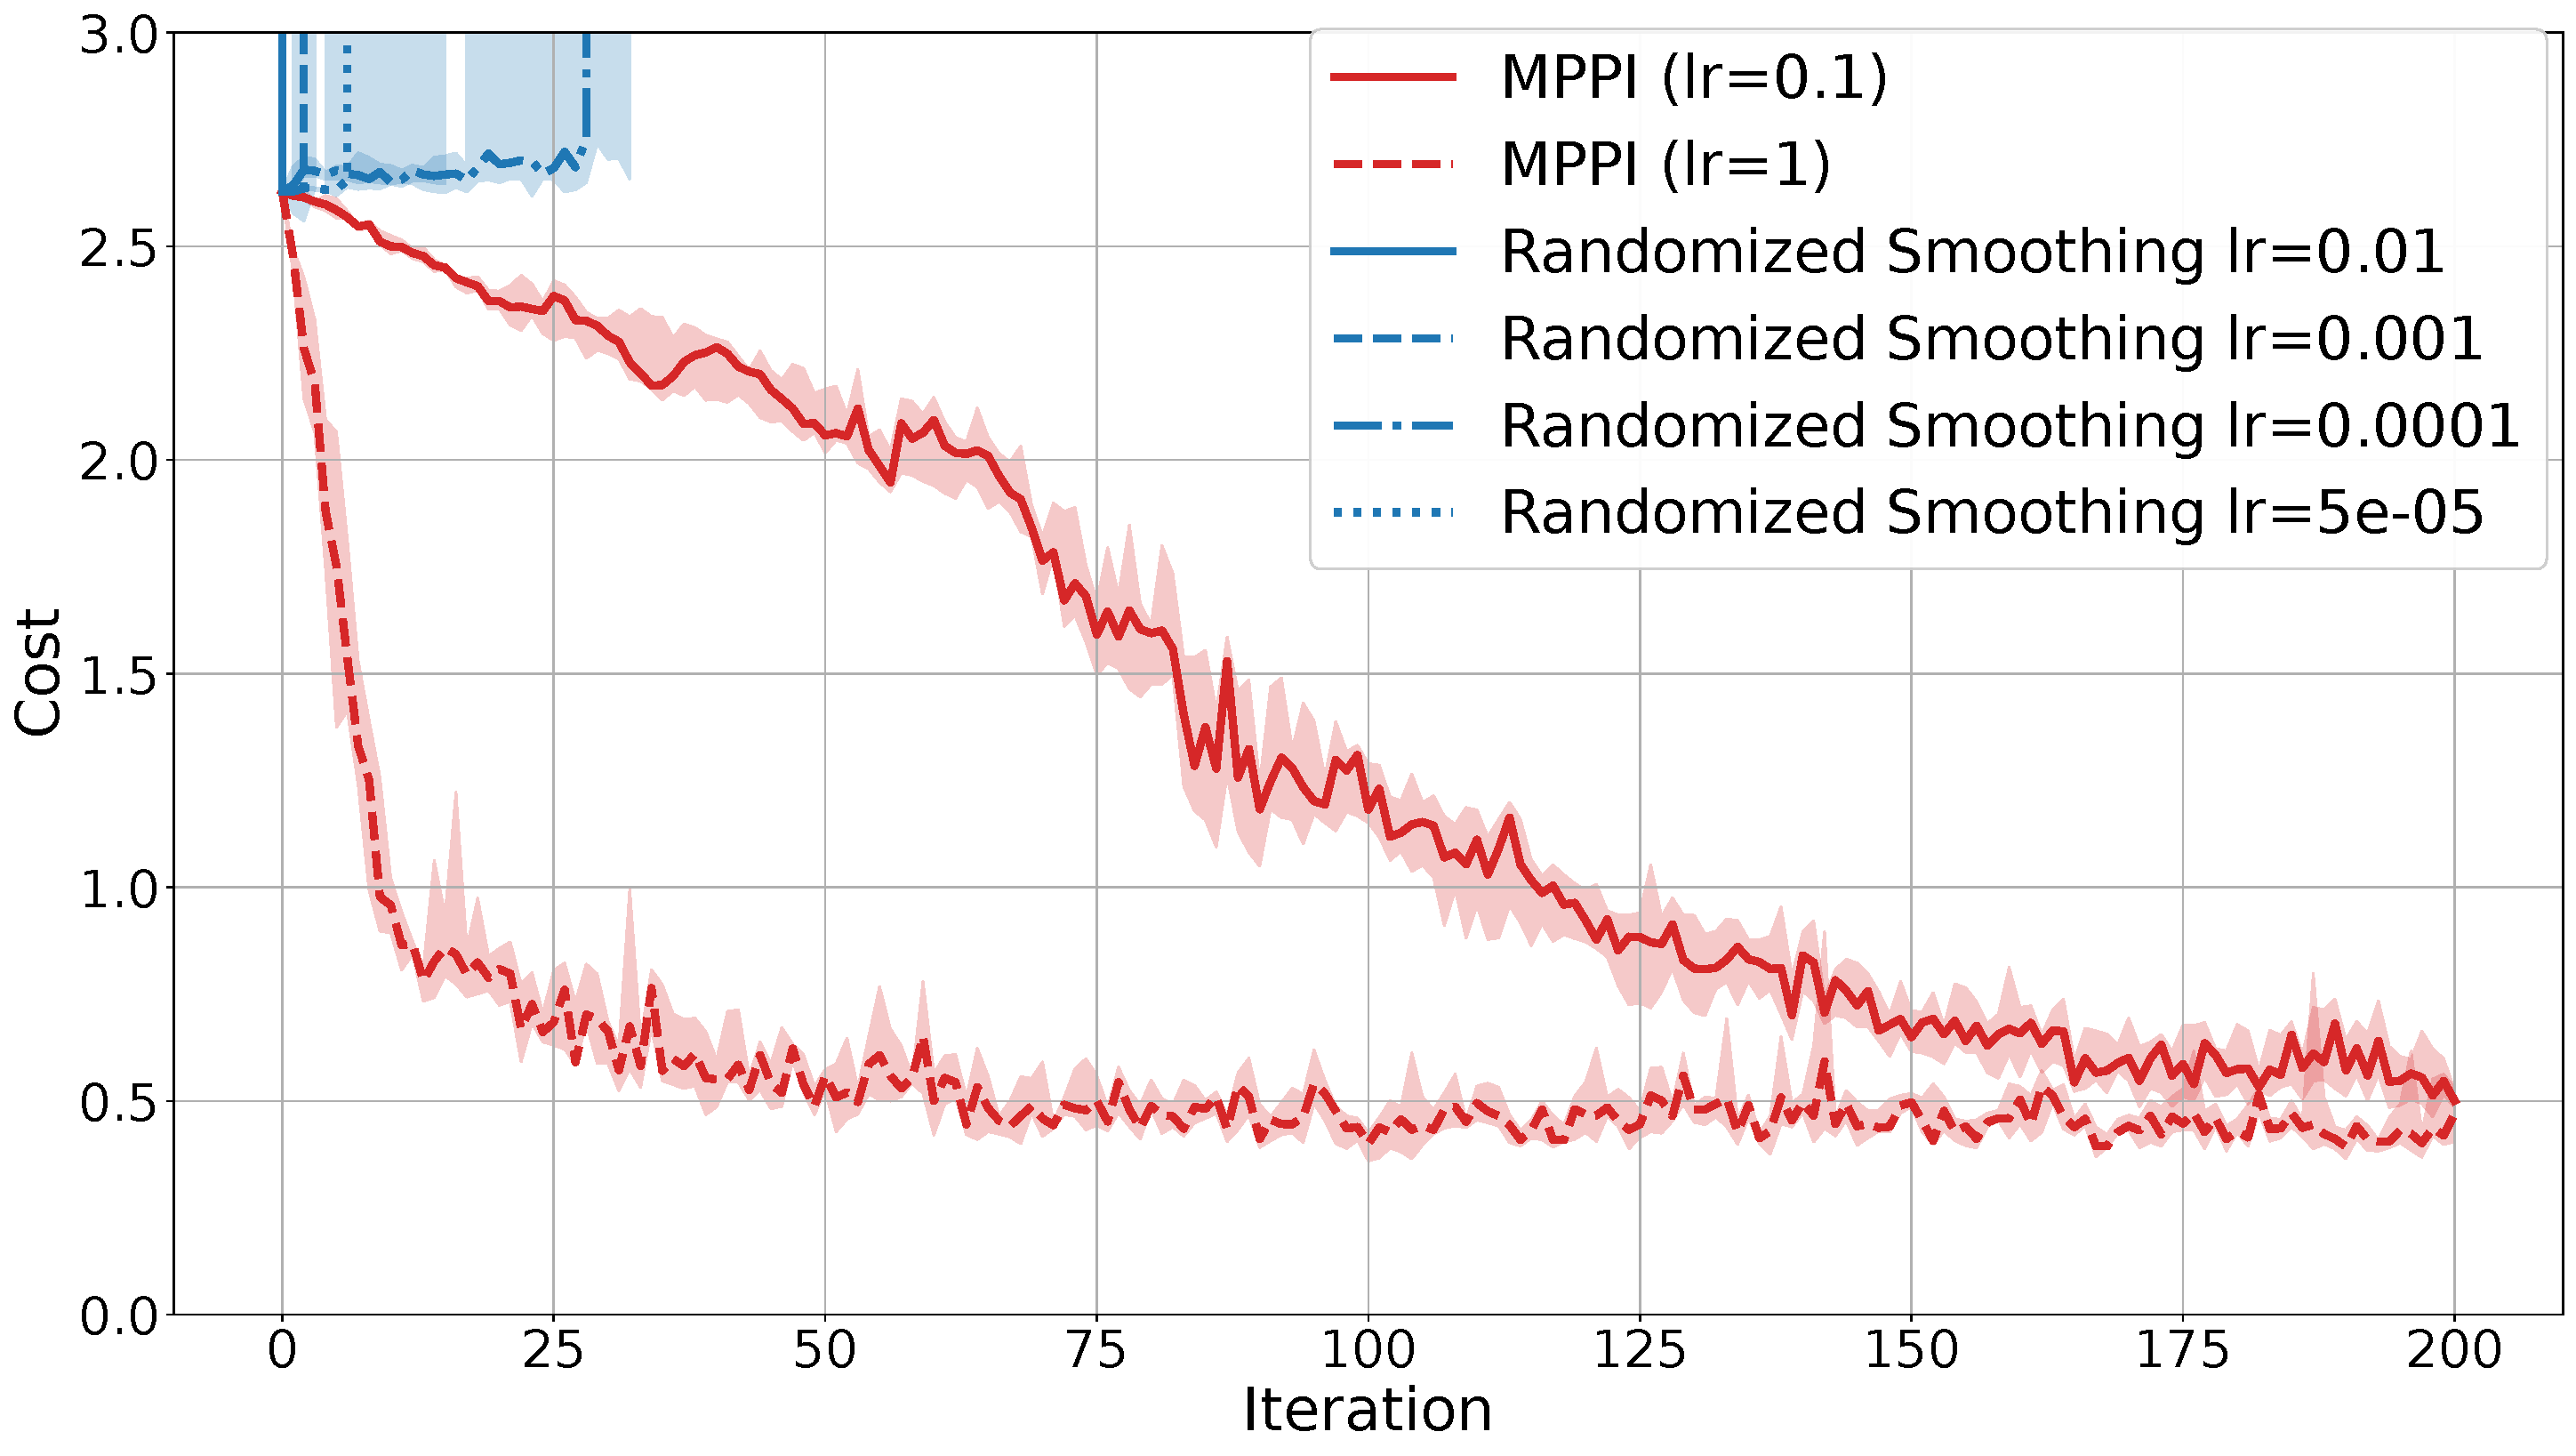
\includegraphics[width=\linewidth]{Go2WalkUnconstrained_Fig1_lr.pdf}
  \caption{Go2Walk}\end{subfigure}\hfill
\begin{subfigure}{0.49\linewidth}\centering
  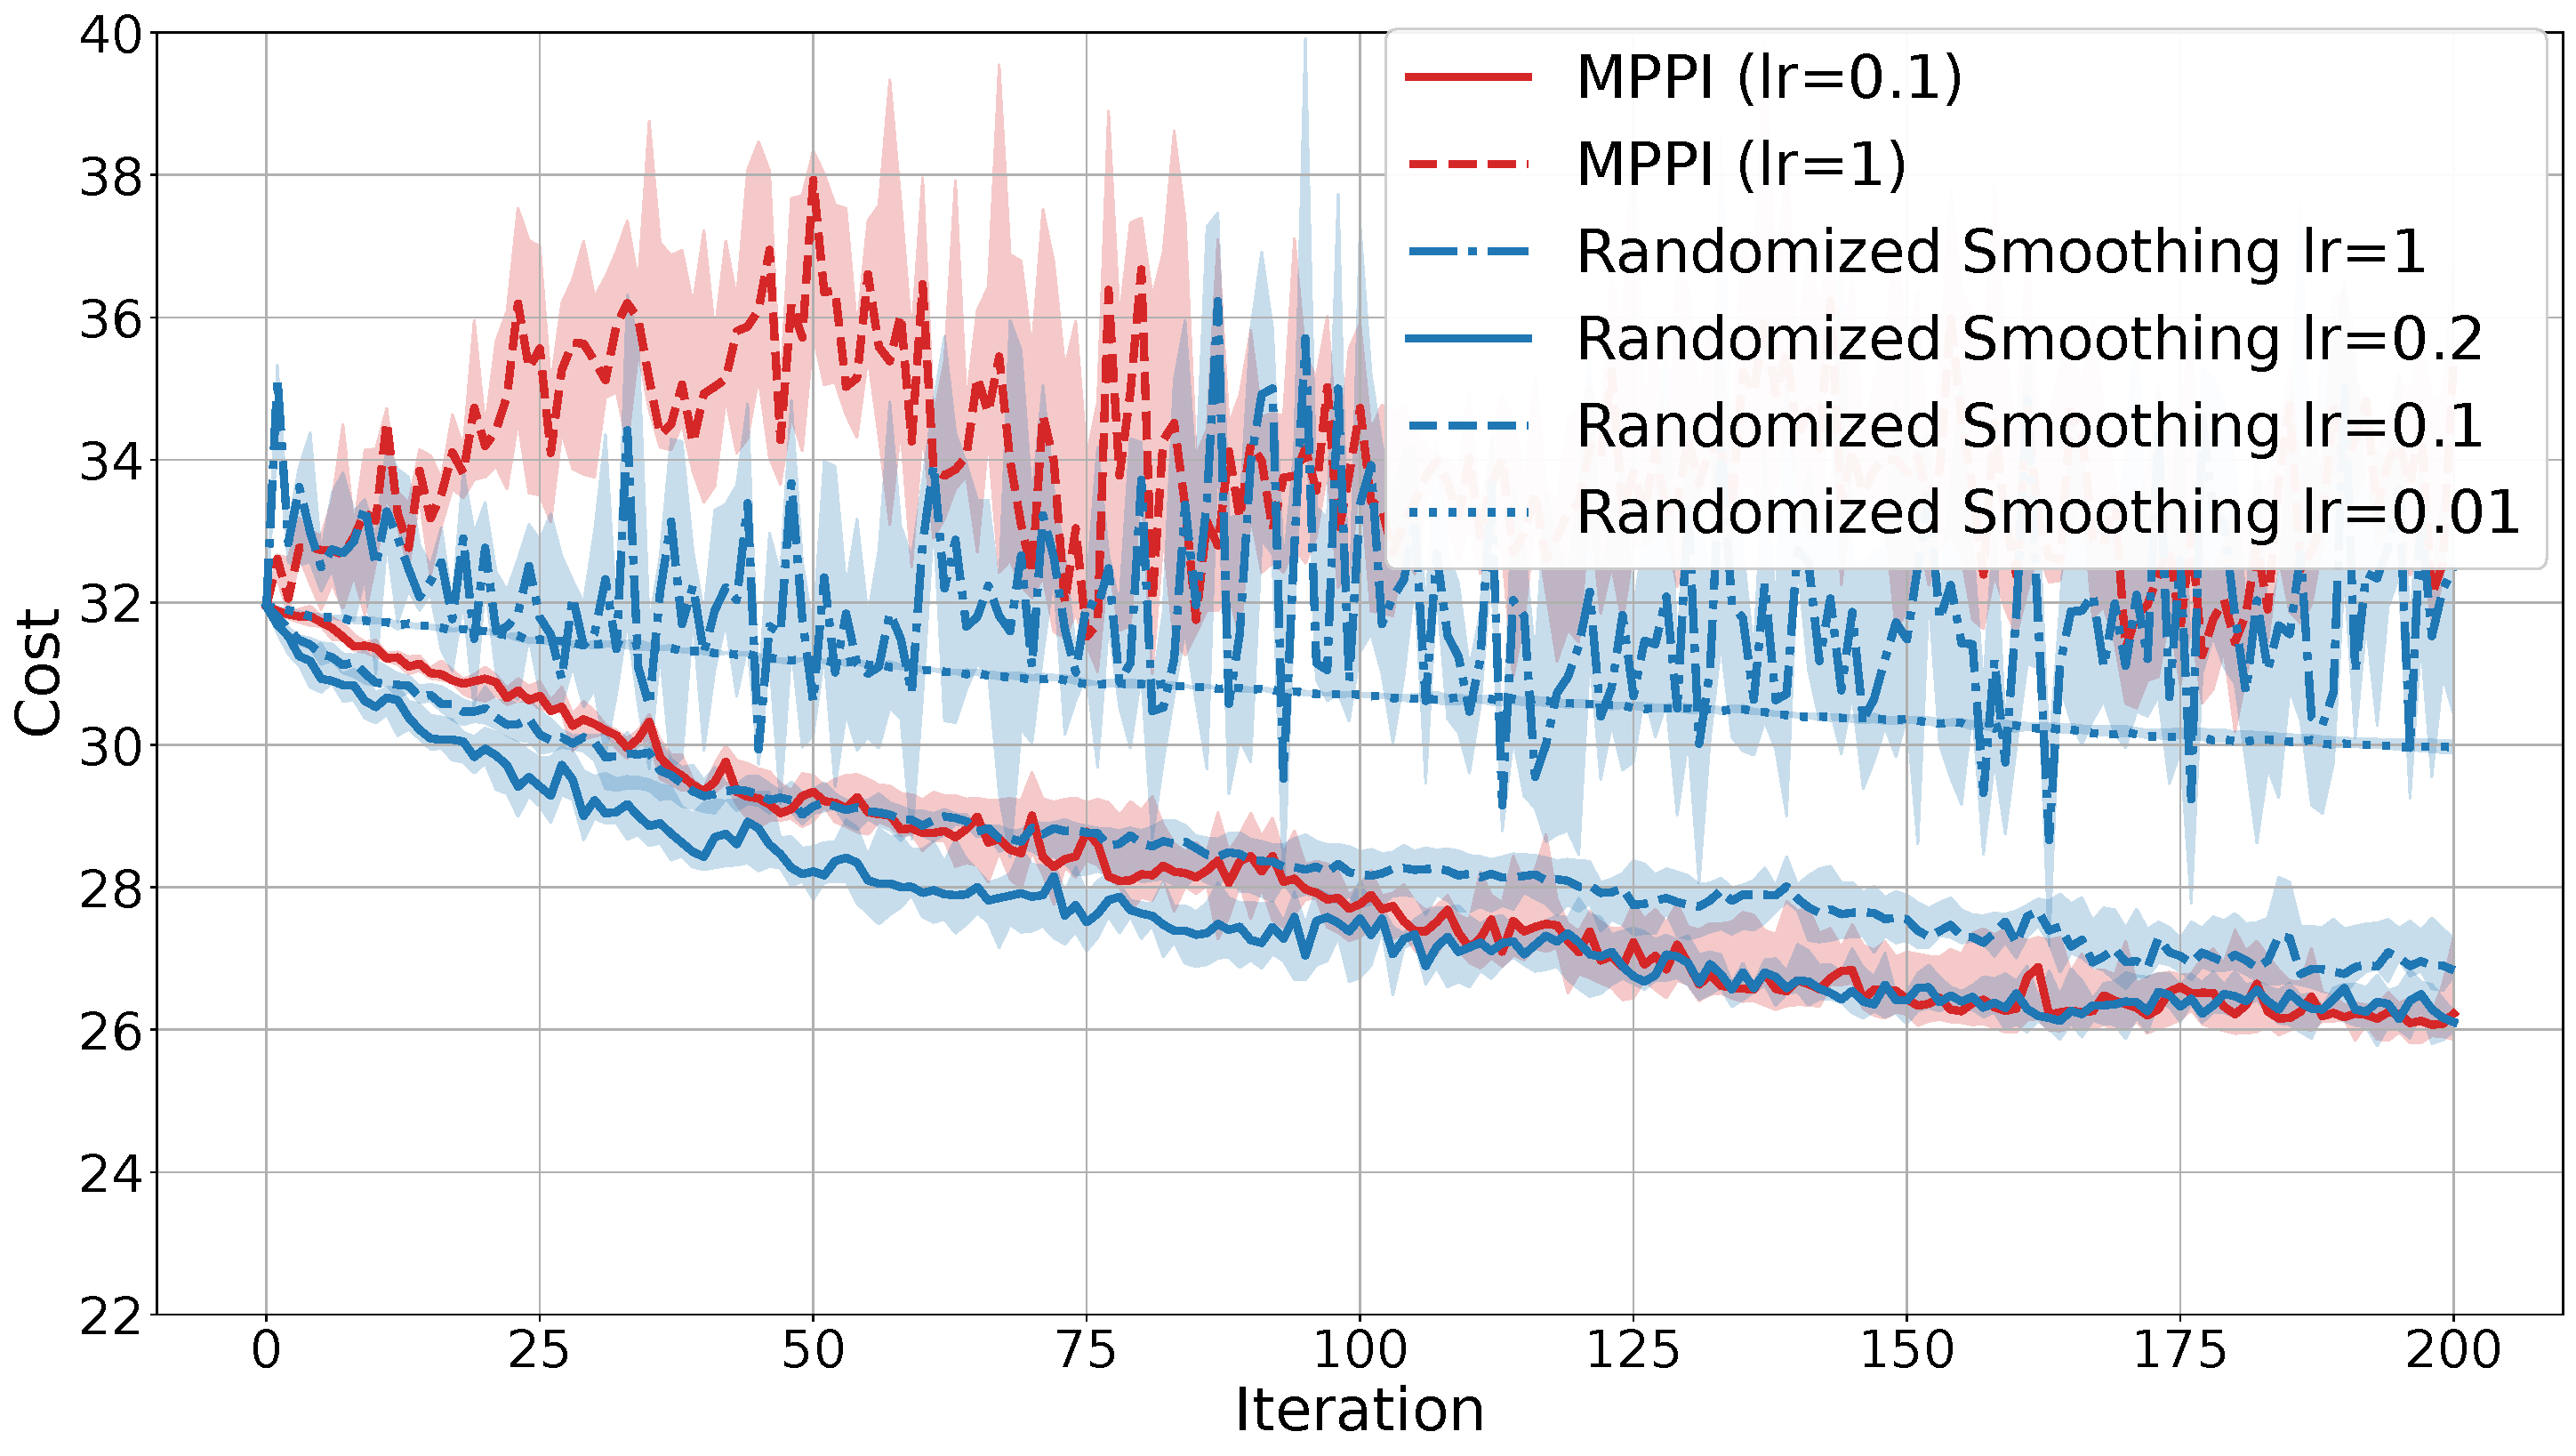
\includegraphics[width=\linewidth]{HumanoidStandupUnconstrained_Fig1_lr.pdf}
  \caption{HumanoidStandup}\end{subfigure}
\caption{Vanilla methods need learning-rate tuning: the best MPPI learning rate is task-dependent (vanilla lr=1 is best on Go2Walk but unstable on HumanoidStandup, where lr=0.1 is needed), and Randomized Smoothing's best LR likewise varies by task (it diverges at every LR on Go2Walk).}
\end{figure}

\begin{figure}[H]
\centering
\begin{subfigure}{0.49\linewidth}\centering
  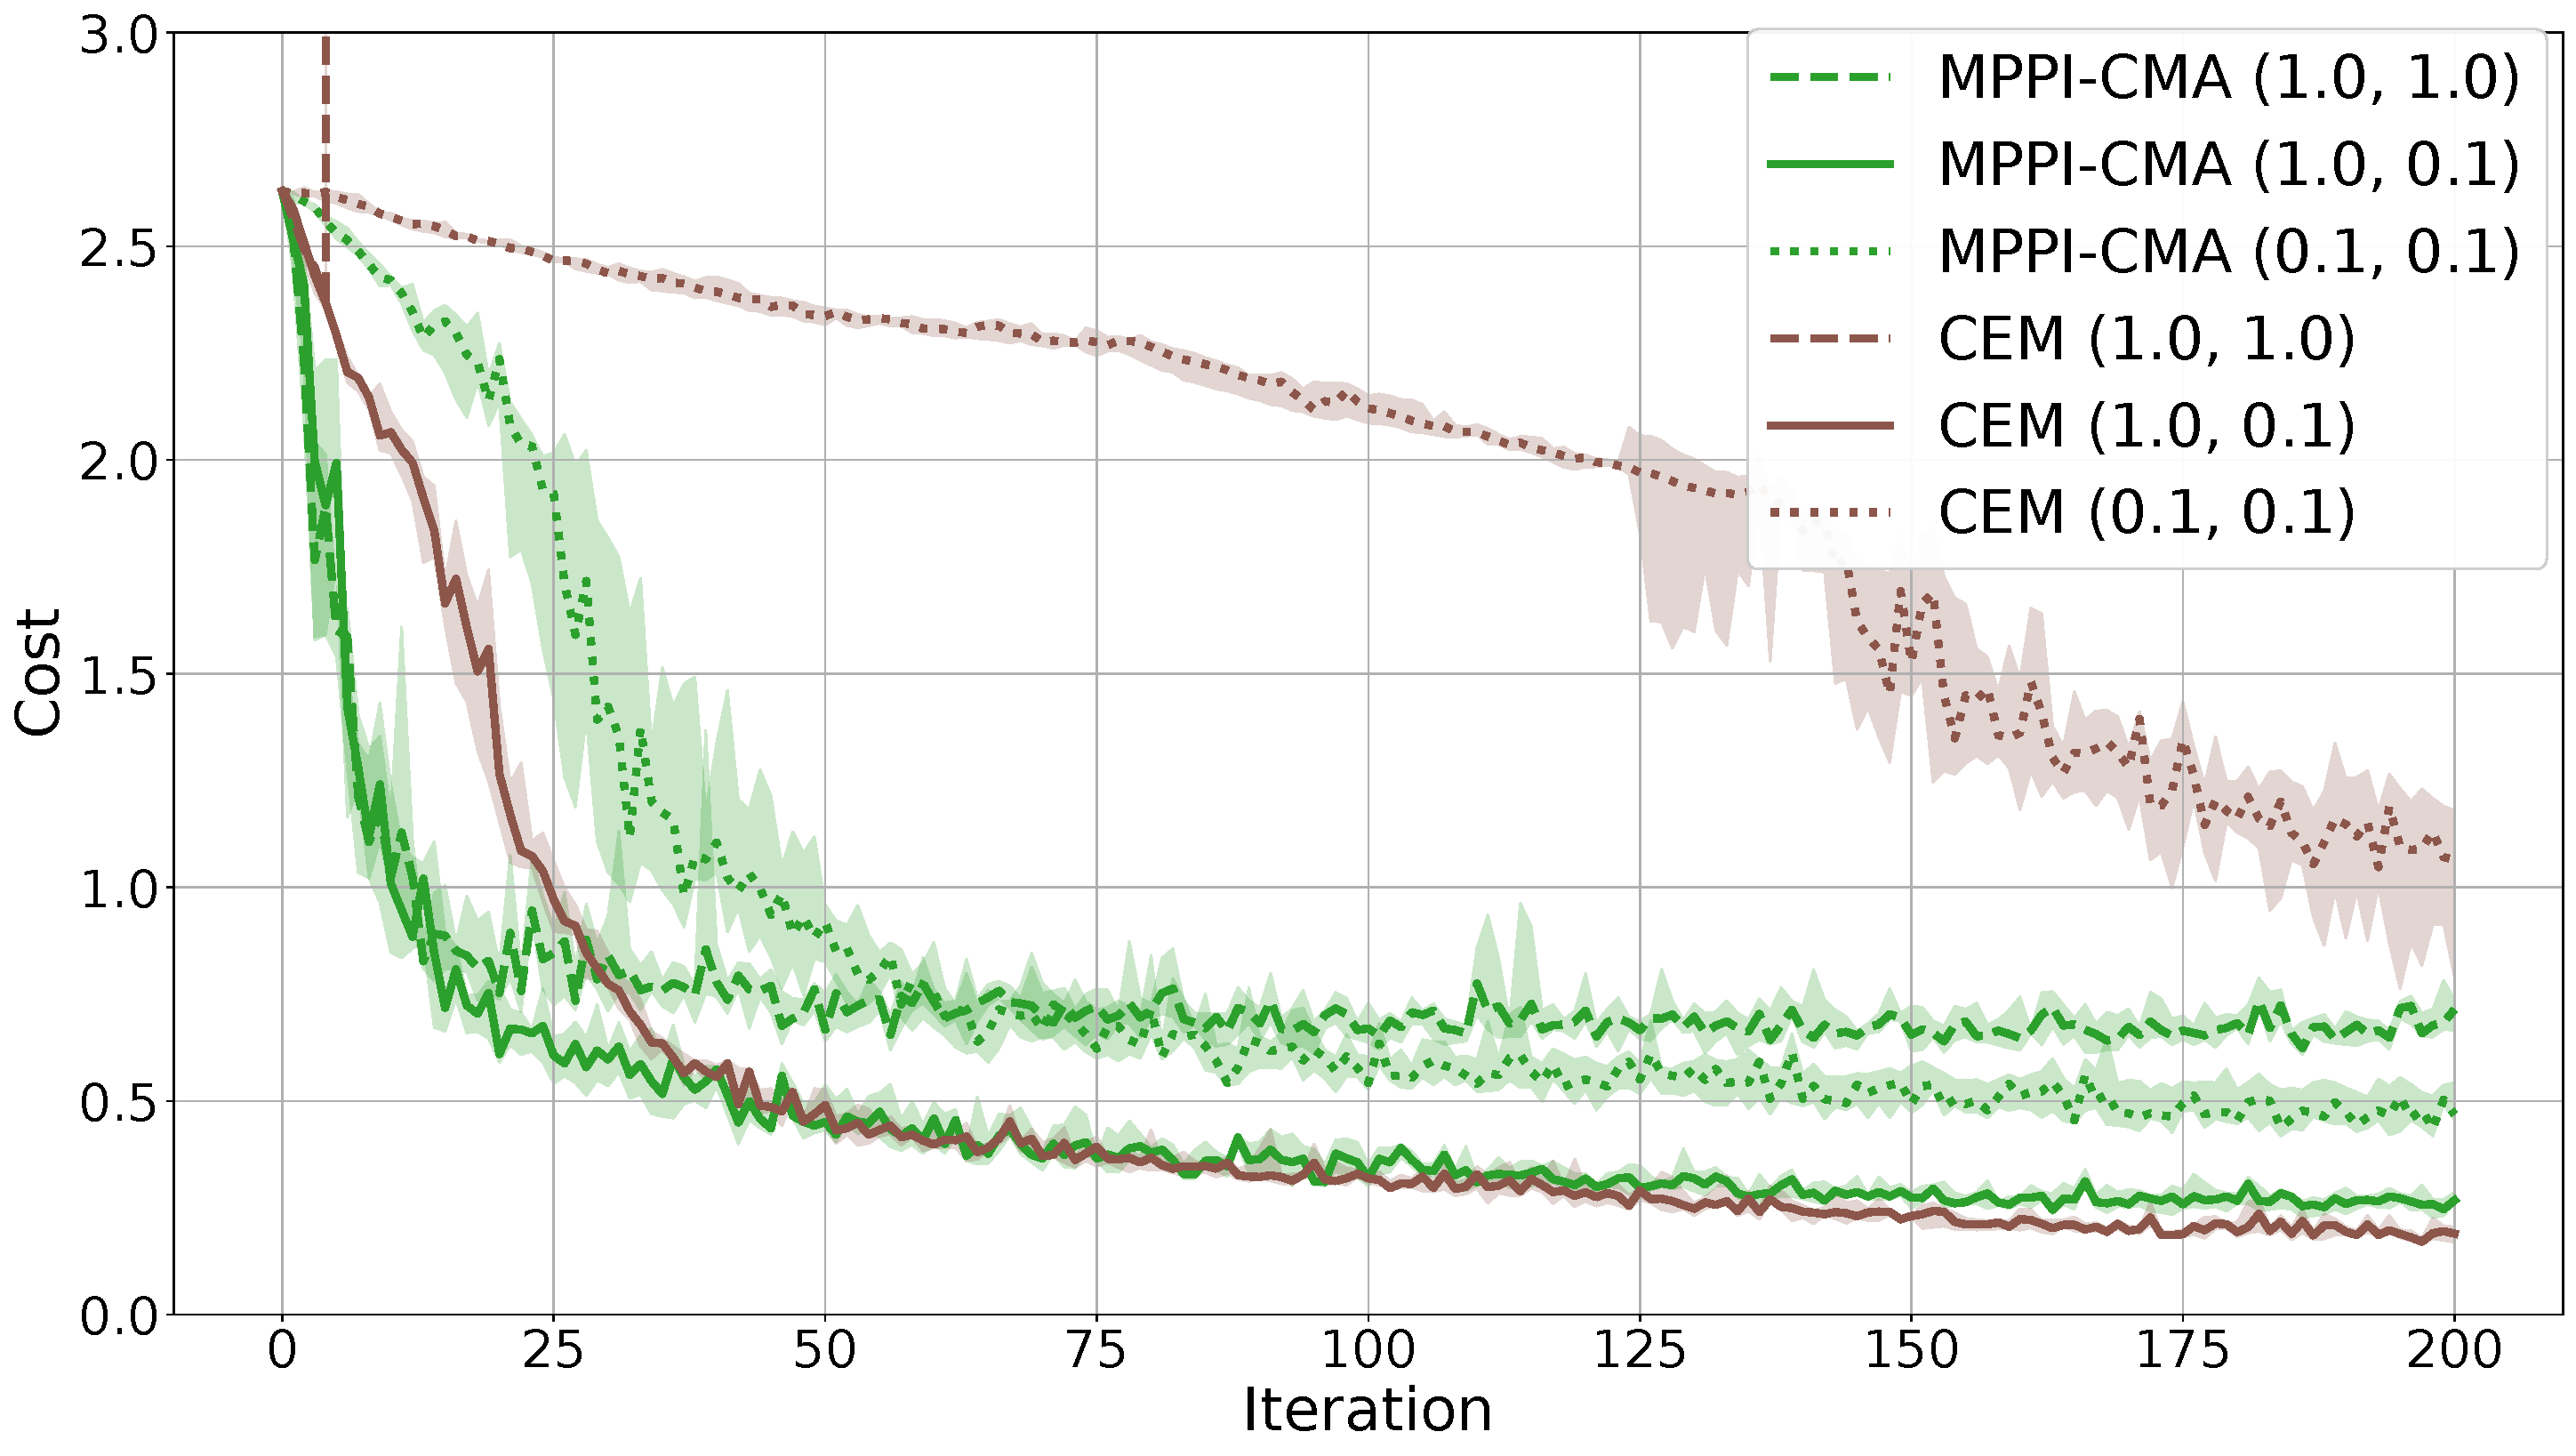
\includegraphics[width=\linewidth]{Go2WalkUnconstrained_Fig2_covlr.pdf}
  \caption{Go2Walk}\end{subfigure}\hfill
\begin{subfigure}{0.49\linewidth}\centering
  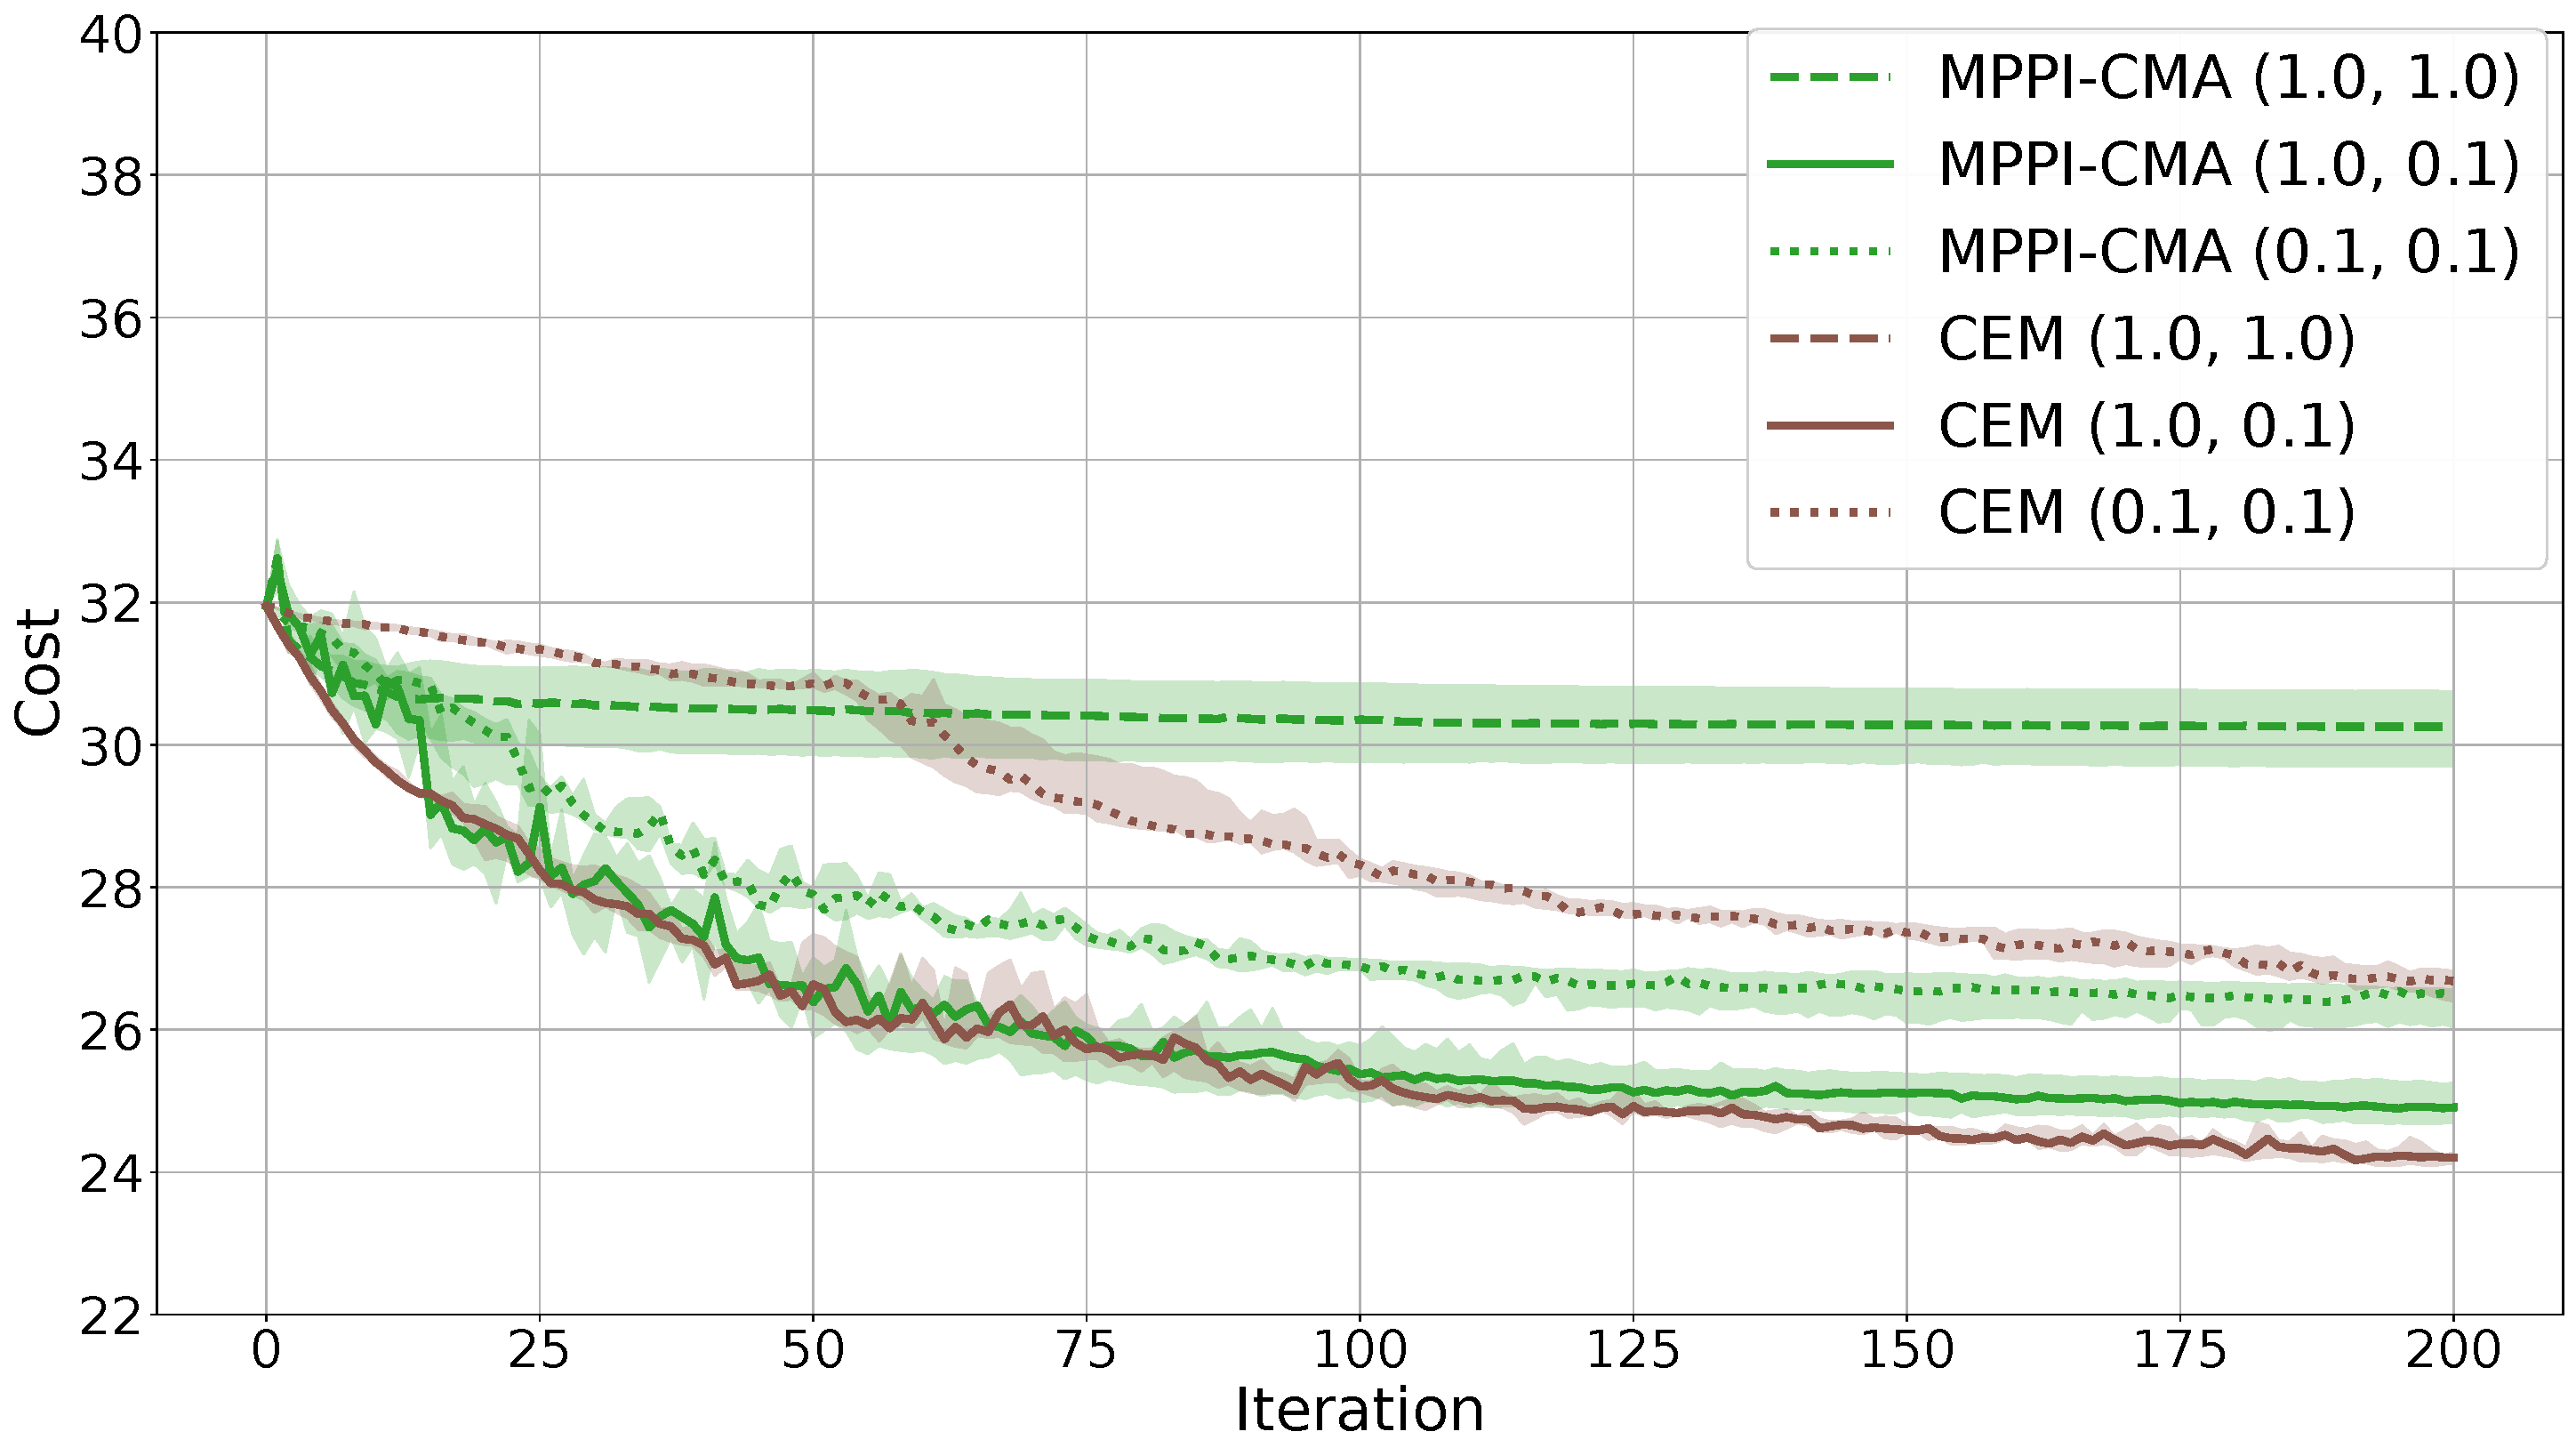
\includegraphics[width=\linewidth]{HumanoidStandupUnconstrained_Fig2_covlr.pdf}
  \caption{HumanoidStandup}\end{subfigure}
\caption{Covariance adaptation needs two distinct learning rates: for both MPPI-CMA and CEM, $(\mathrm{mean},\mathrm{cov})=(1,0.1)$ outperforms a single shared rate $(1,1)$ or $(0.1,0.1)$ on both Go2Walk and HumanoidStandup.}
\end{figure}

\begin{figure}[H]
\centering
\begin{subfigure}{0.49\linewidth}\centering
  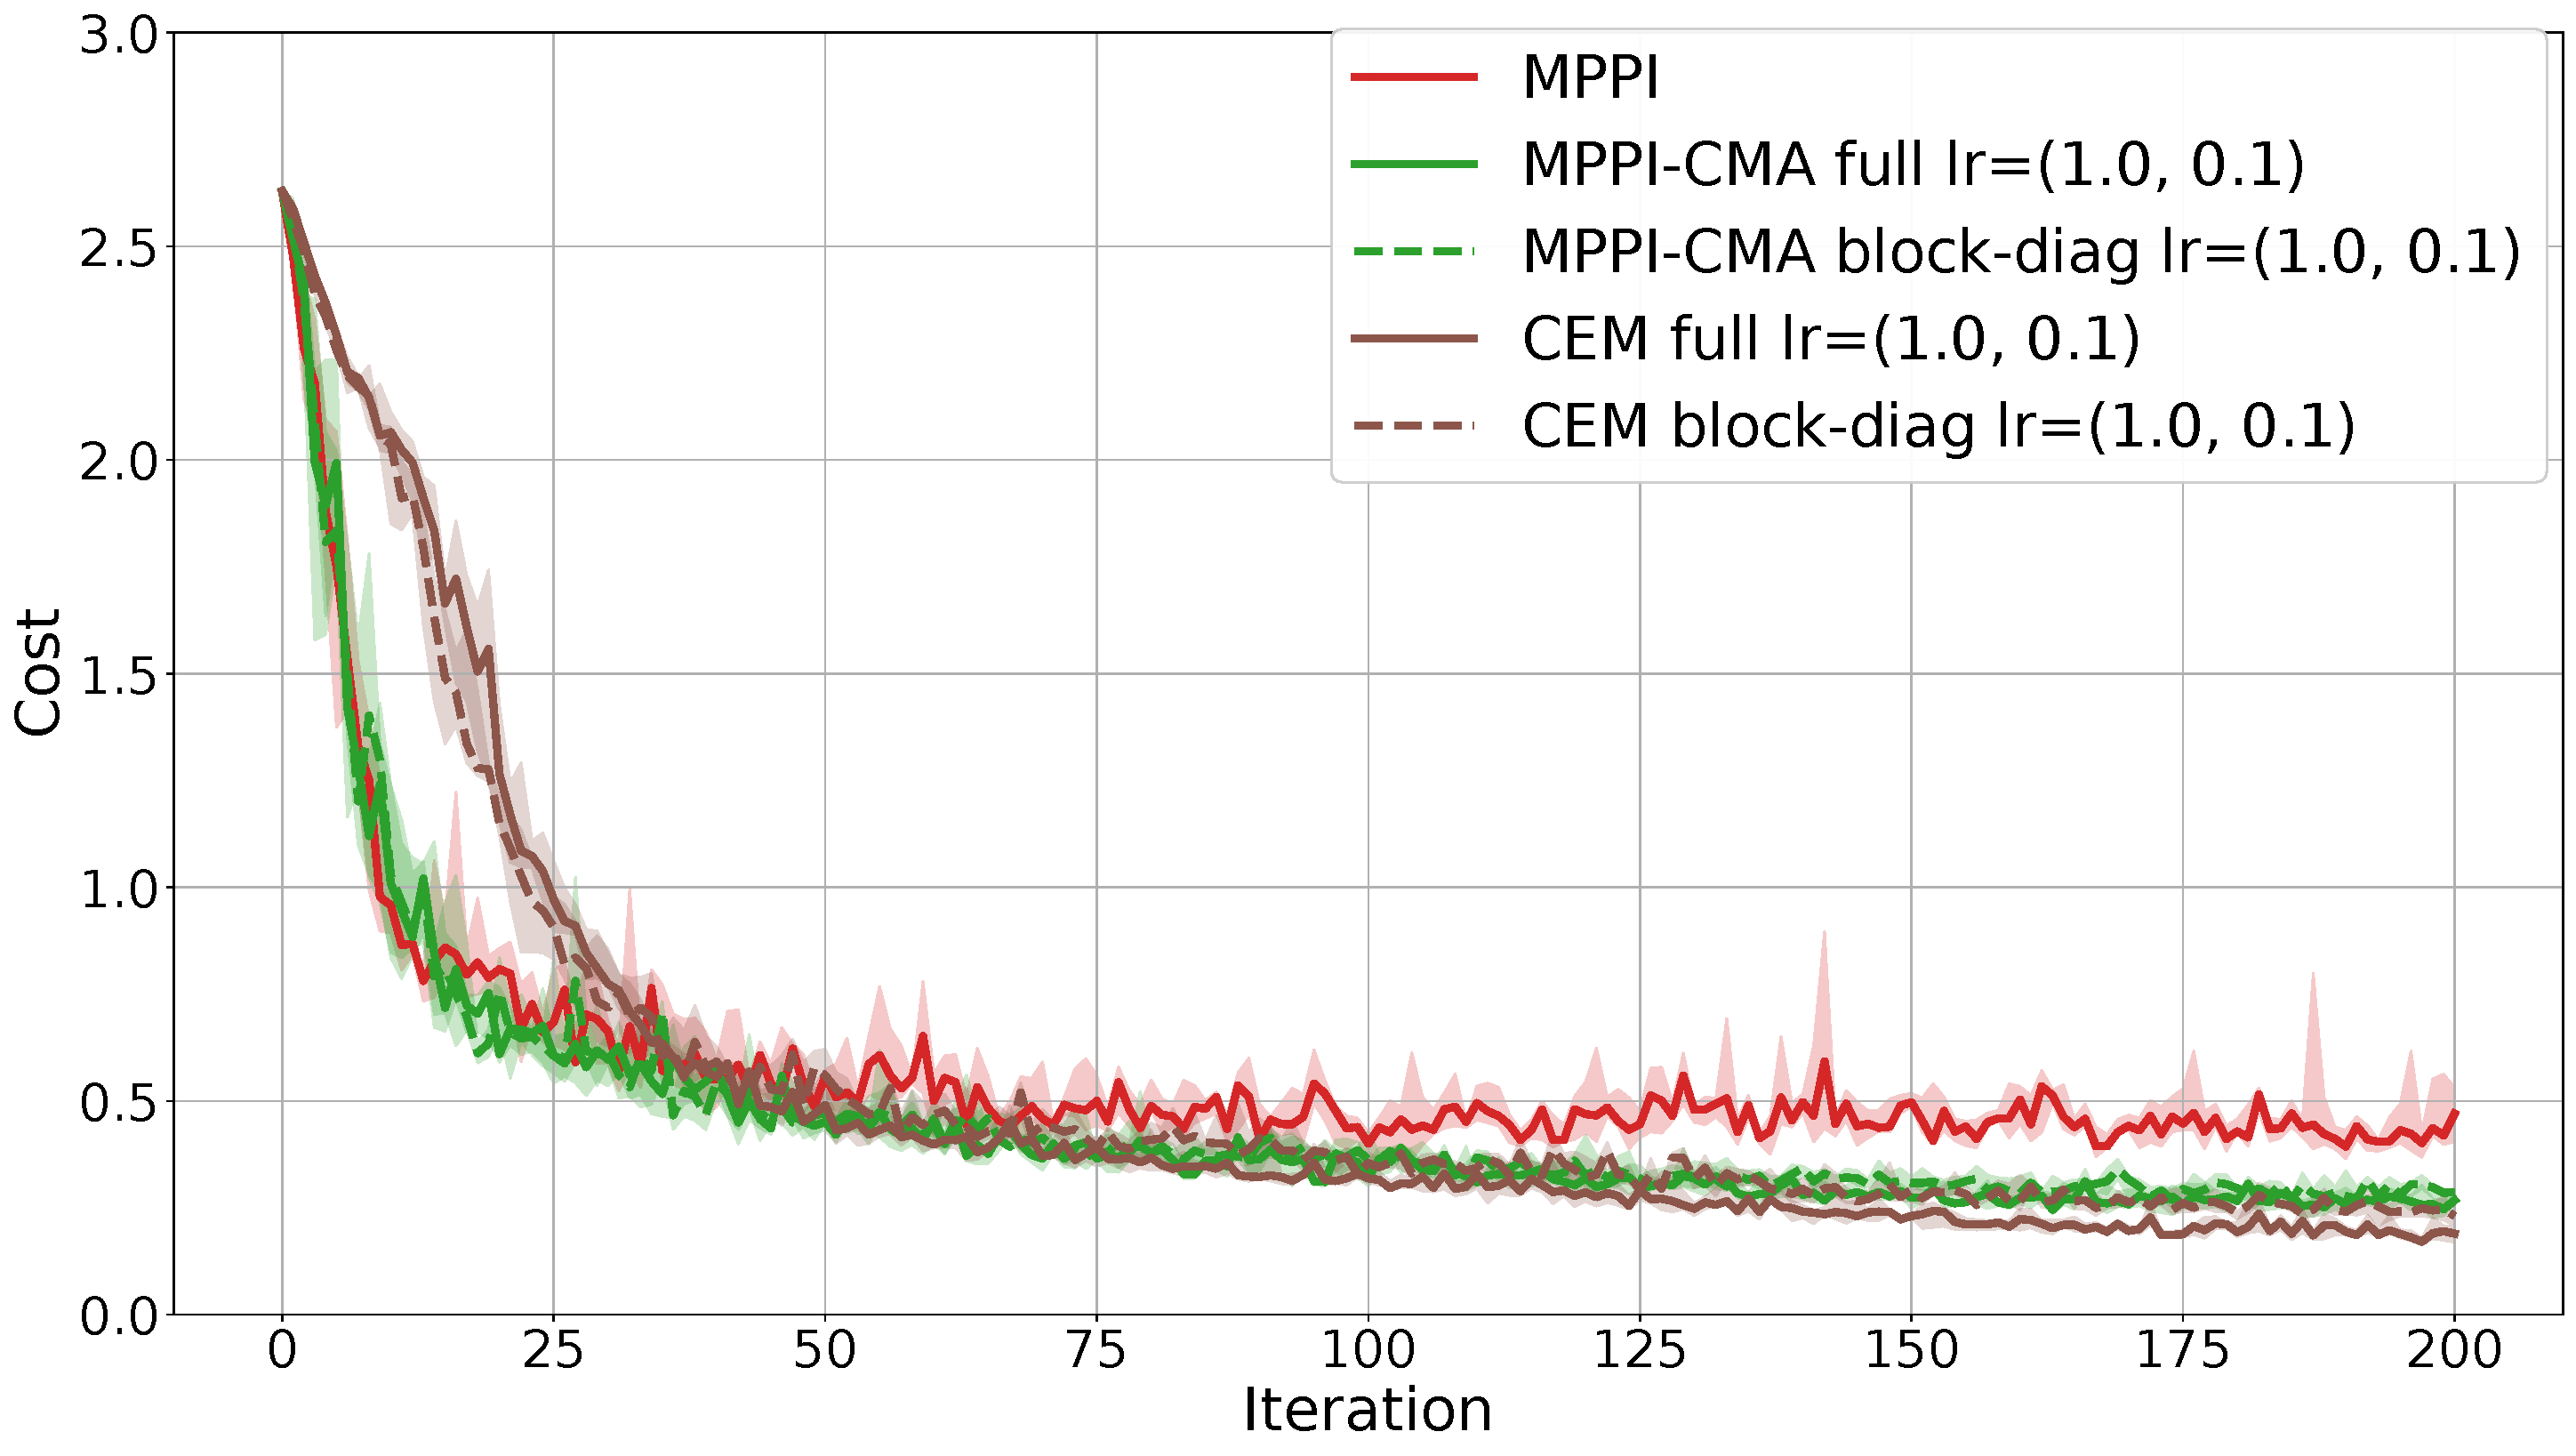
\includegraphics[width=\linewidth]{Go2WalkUnconstrained_Fig3_covhelps.pdf}
  \caption{Go2Walk}\end{subfigure}\hfill
\begin{subfigure}{0.49\linewidth}\centering
  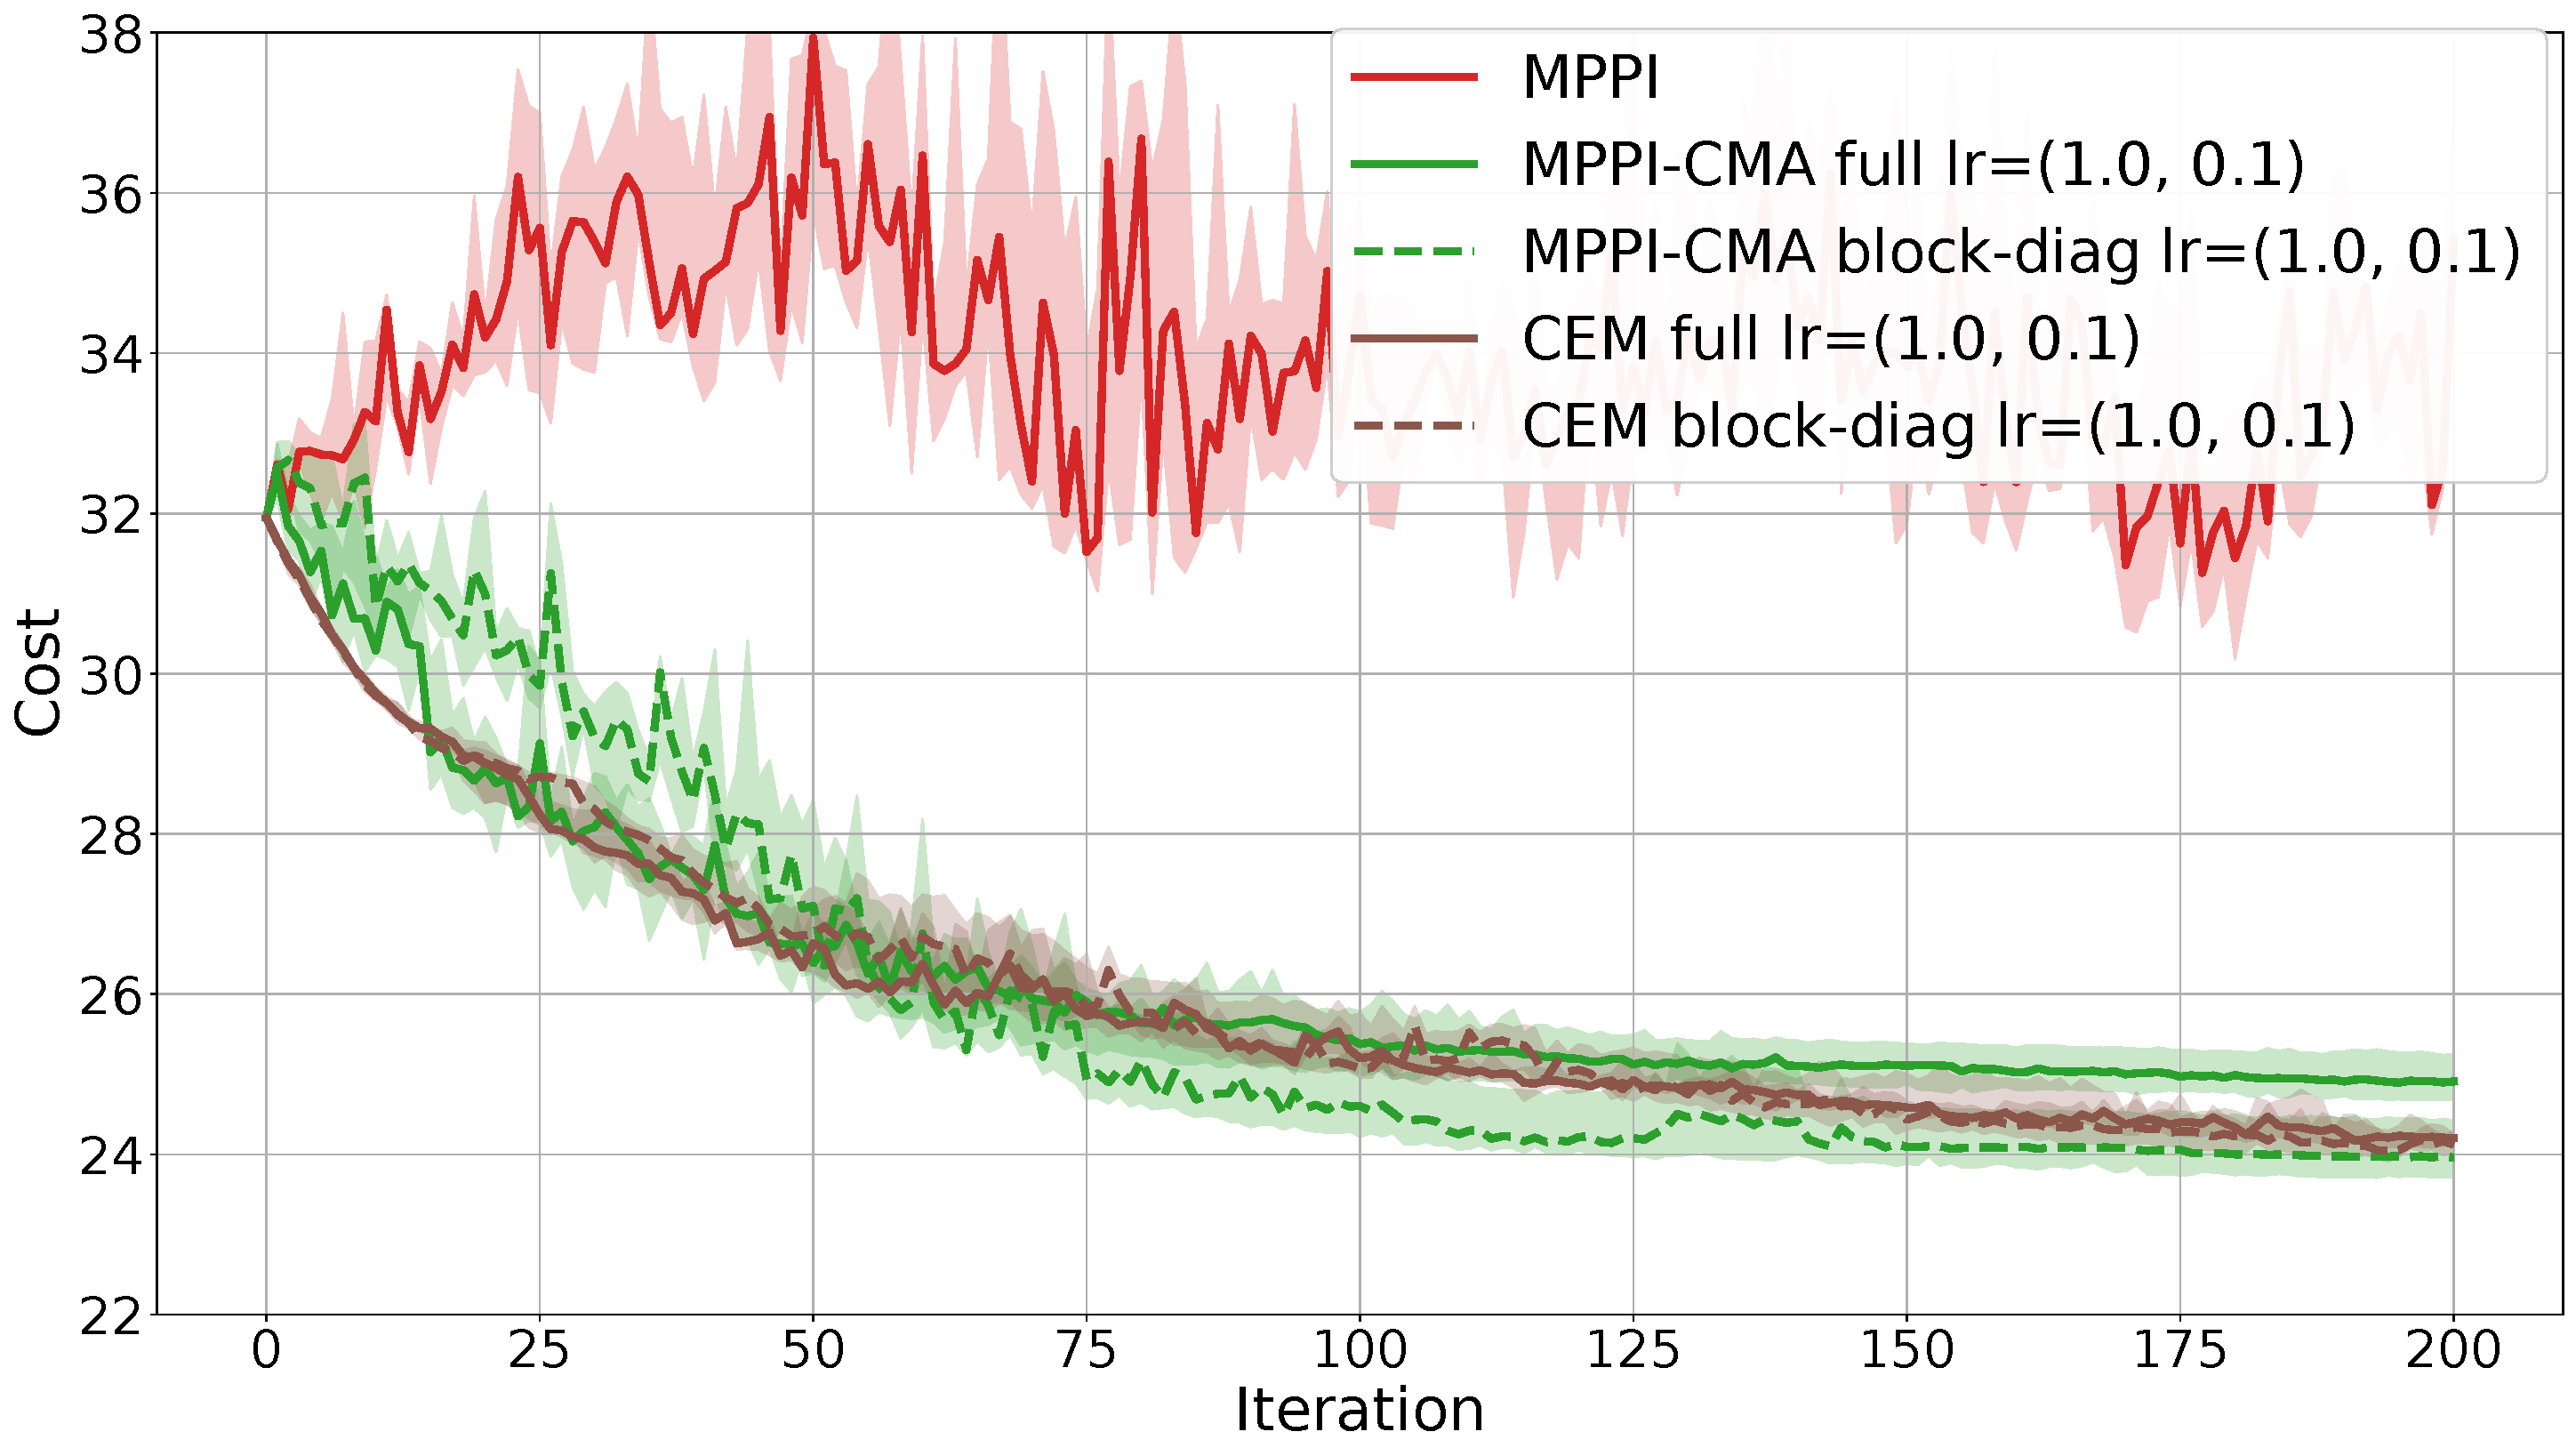
\includegraphics[width=\linewidth]{HumanoidStandupUnconstrained_Fig3_covhelps.pdf}
  \caption{HumanoidStandup}\end{subfigure}
\caption{Covariance adaptation helps and block-diagonal $\approx$ full: MPPI-CMA and CEM (full and block-diagonal) improve over the MPPI baseline on both Go2Walk and HumanoidStandup; block-diagonal closely matches full covariance.}
\end{figure}

% ============================================================
%  Per-task appendix figure (6 tasks, 7-algorithm full set), 3x2 grid
% ============================================================
\begin{figure}[H]
\centering
% top row: classic / easier
\begin{subfigure}{0.32\textwidth}\centering
  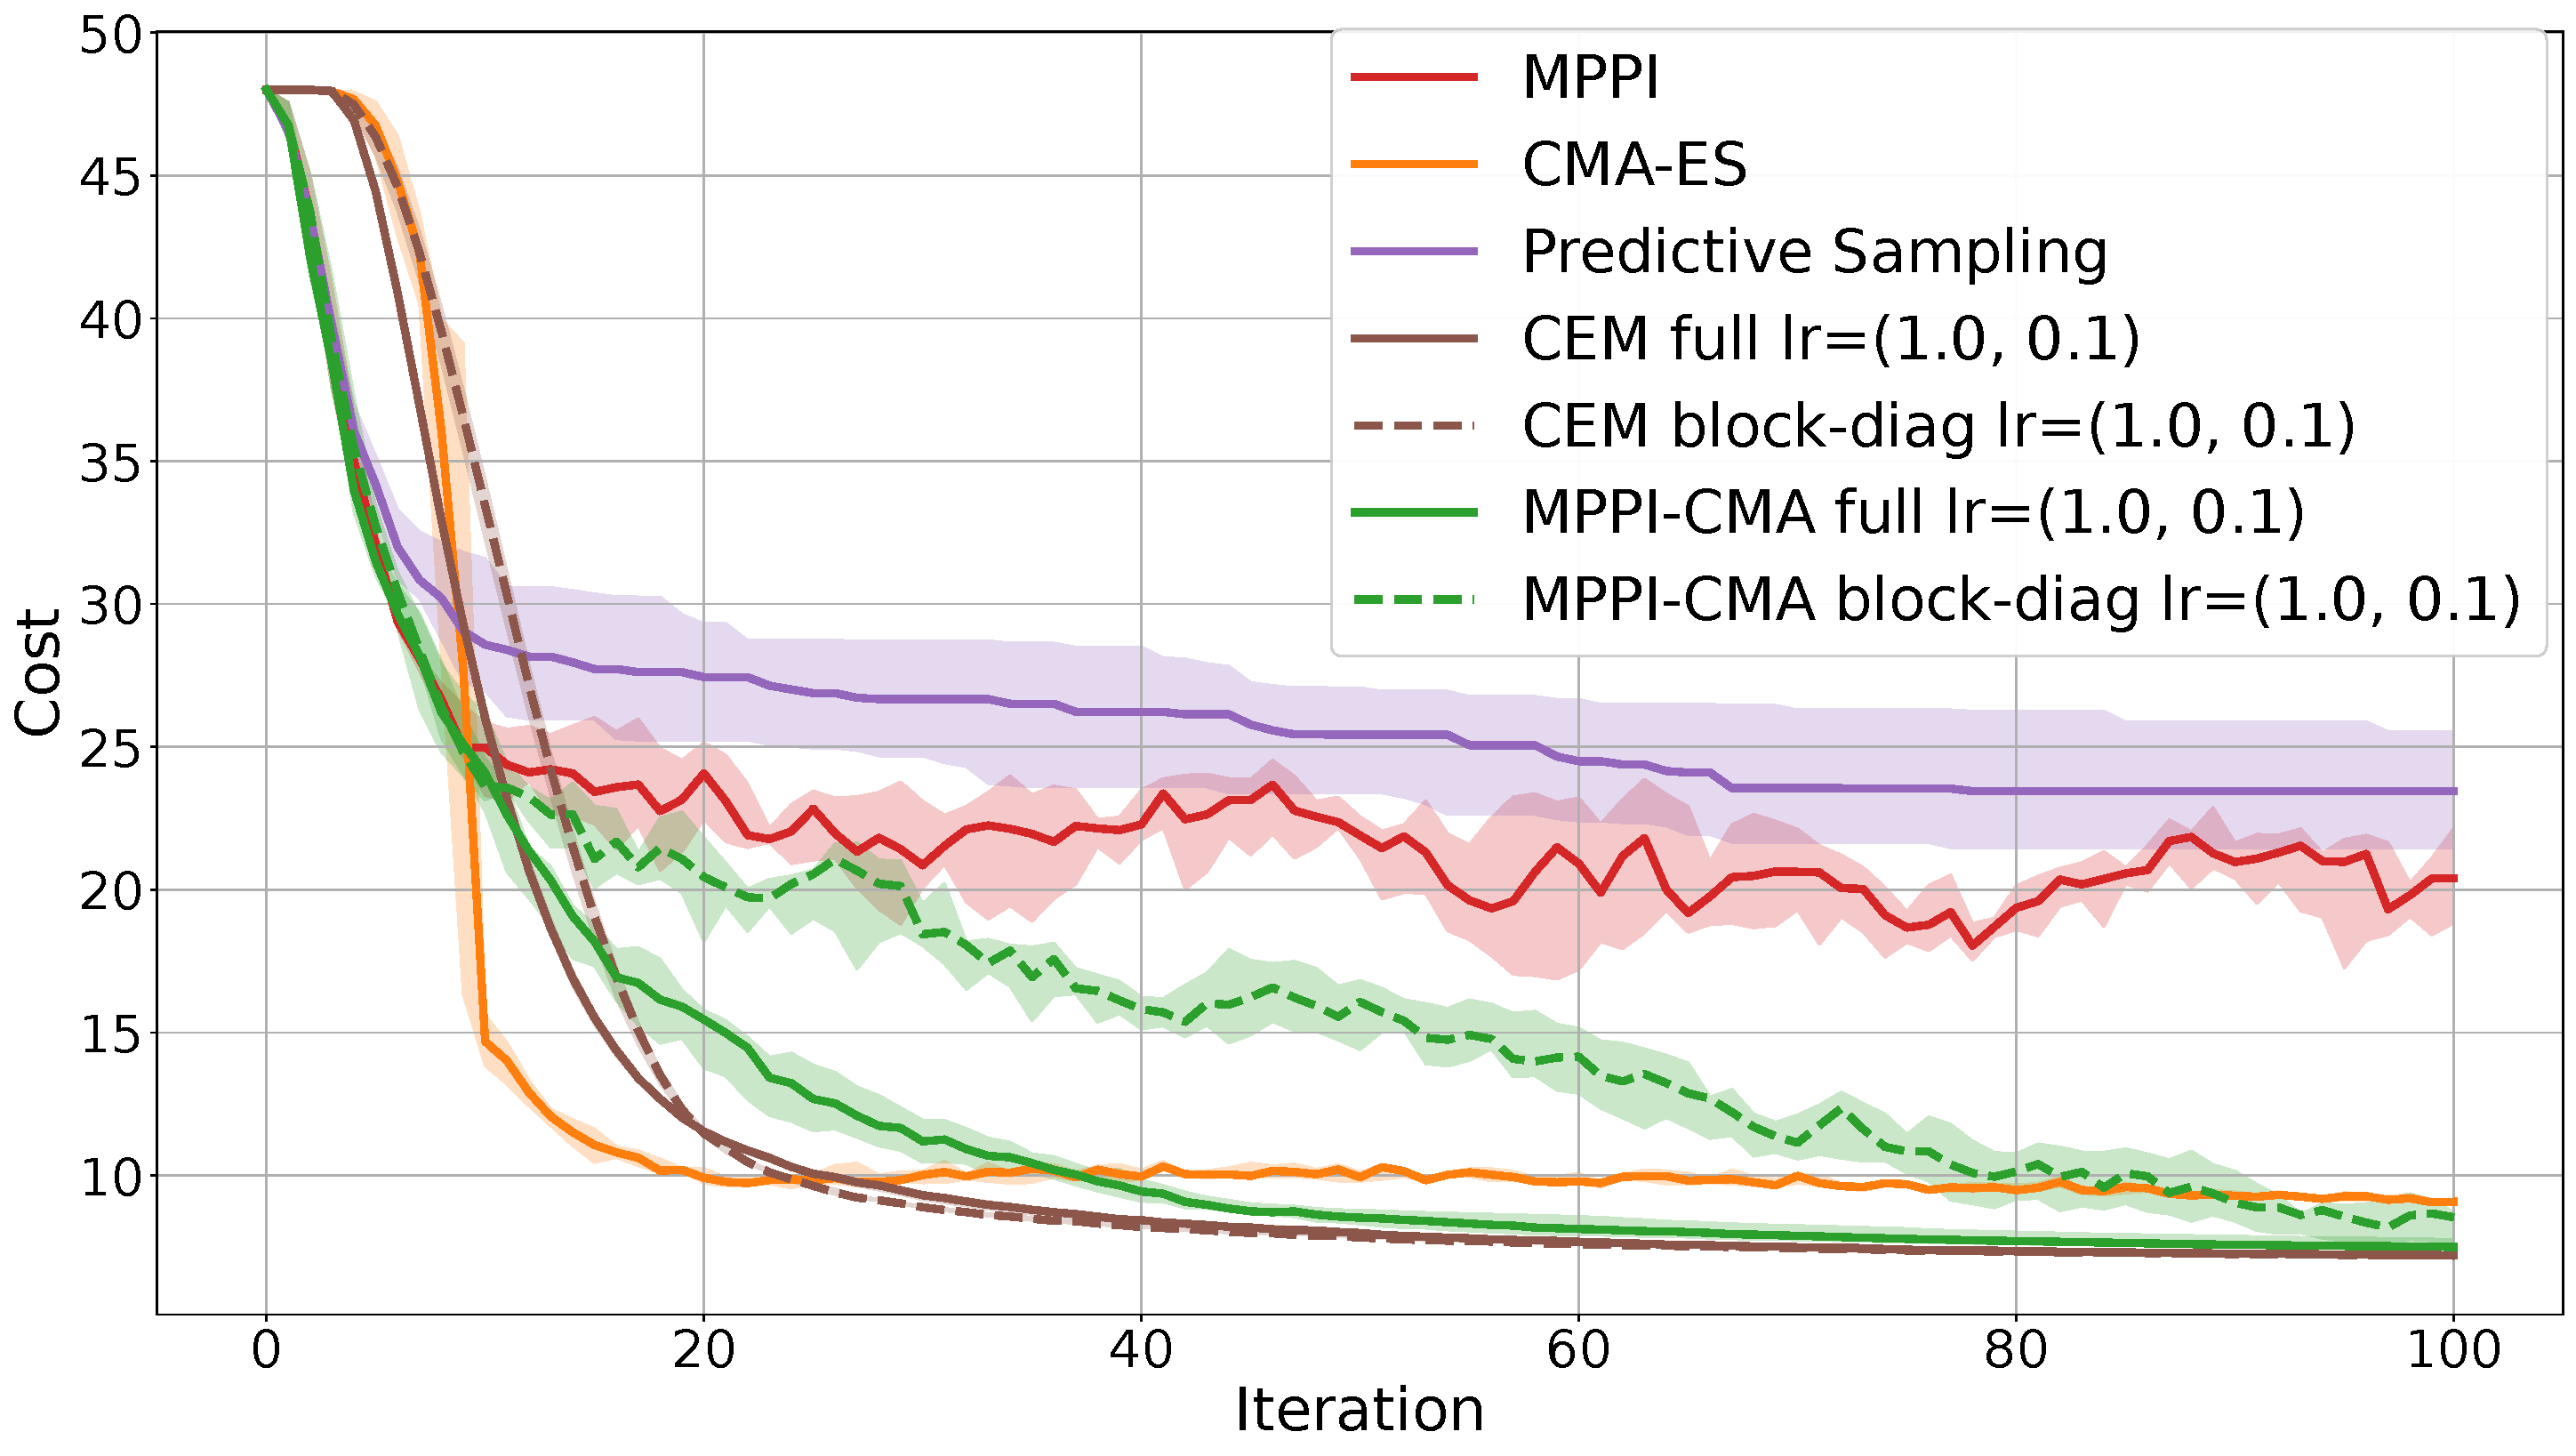
\includegraphics[width=\linewidth]{CartPoleUnconstrained_Convergence_full.pdf}
  \caption{CartPole}\end{subfigure}\hfill
\begin{subfigure}{0.32\textwidth}\centering
  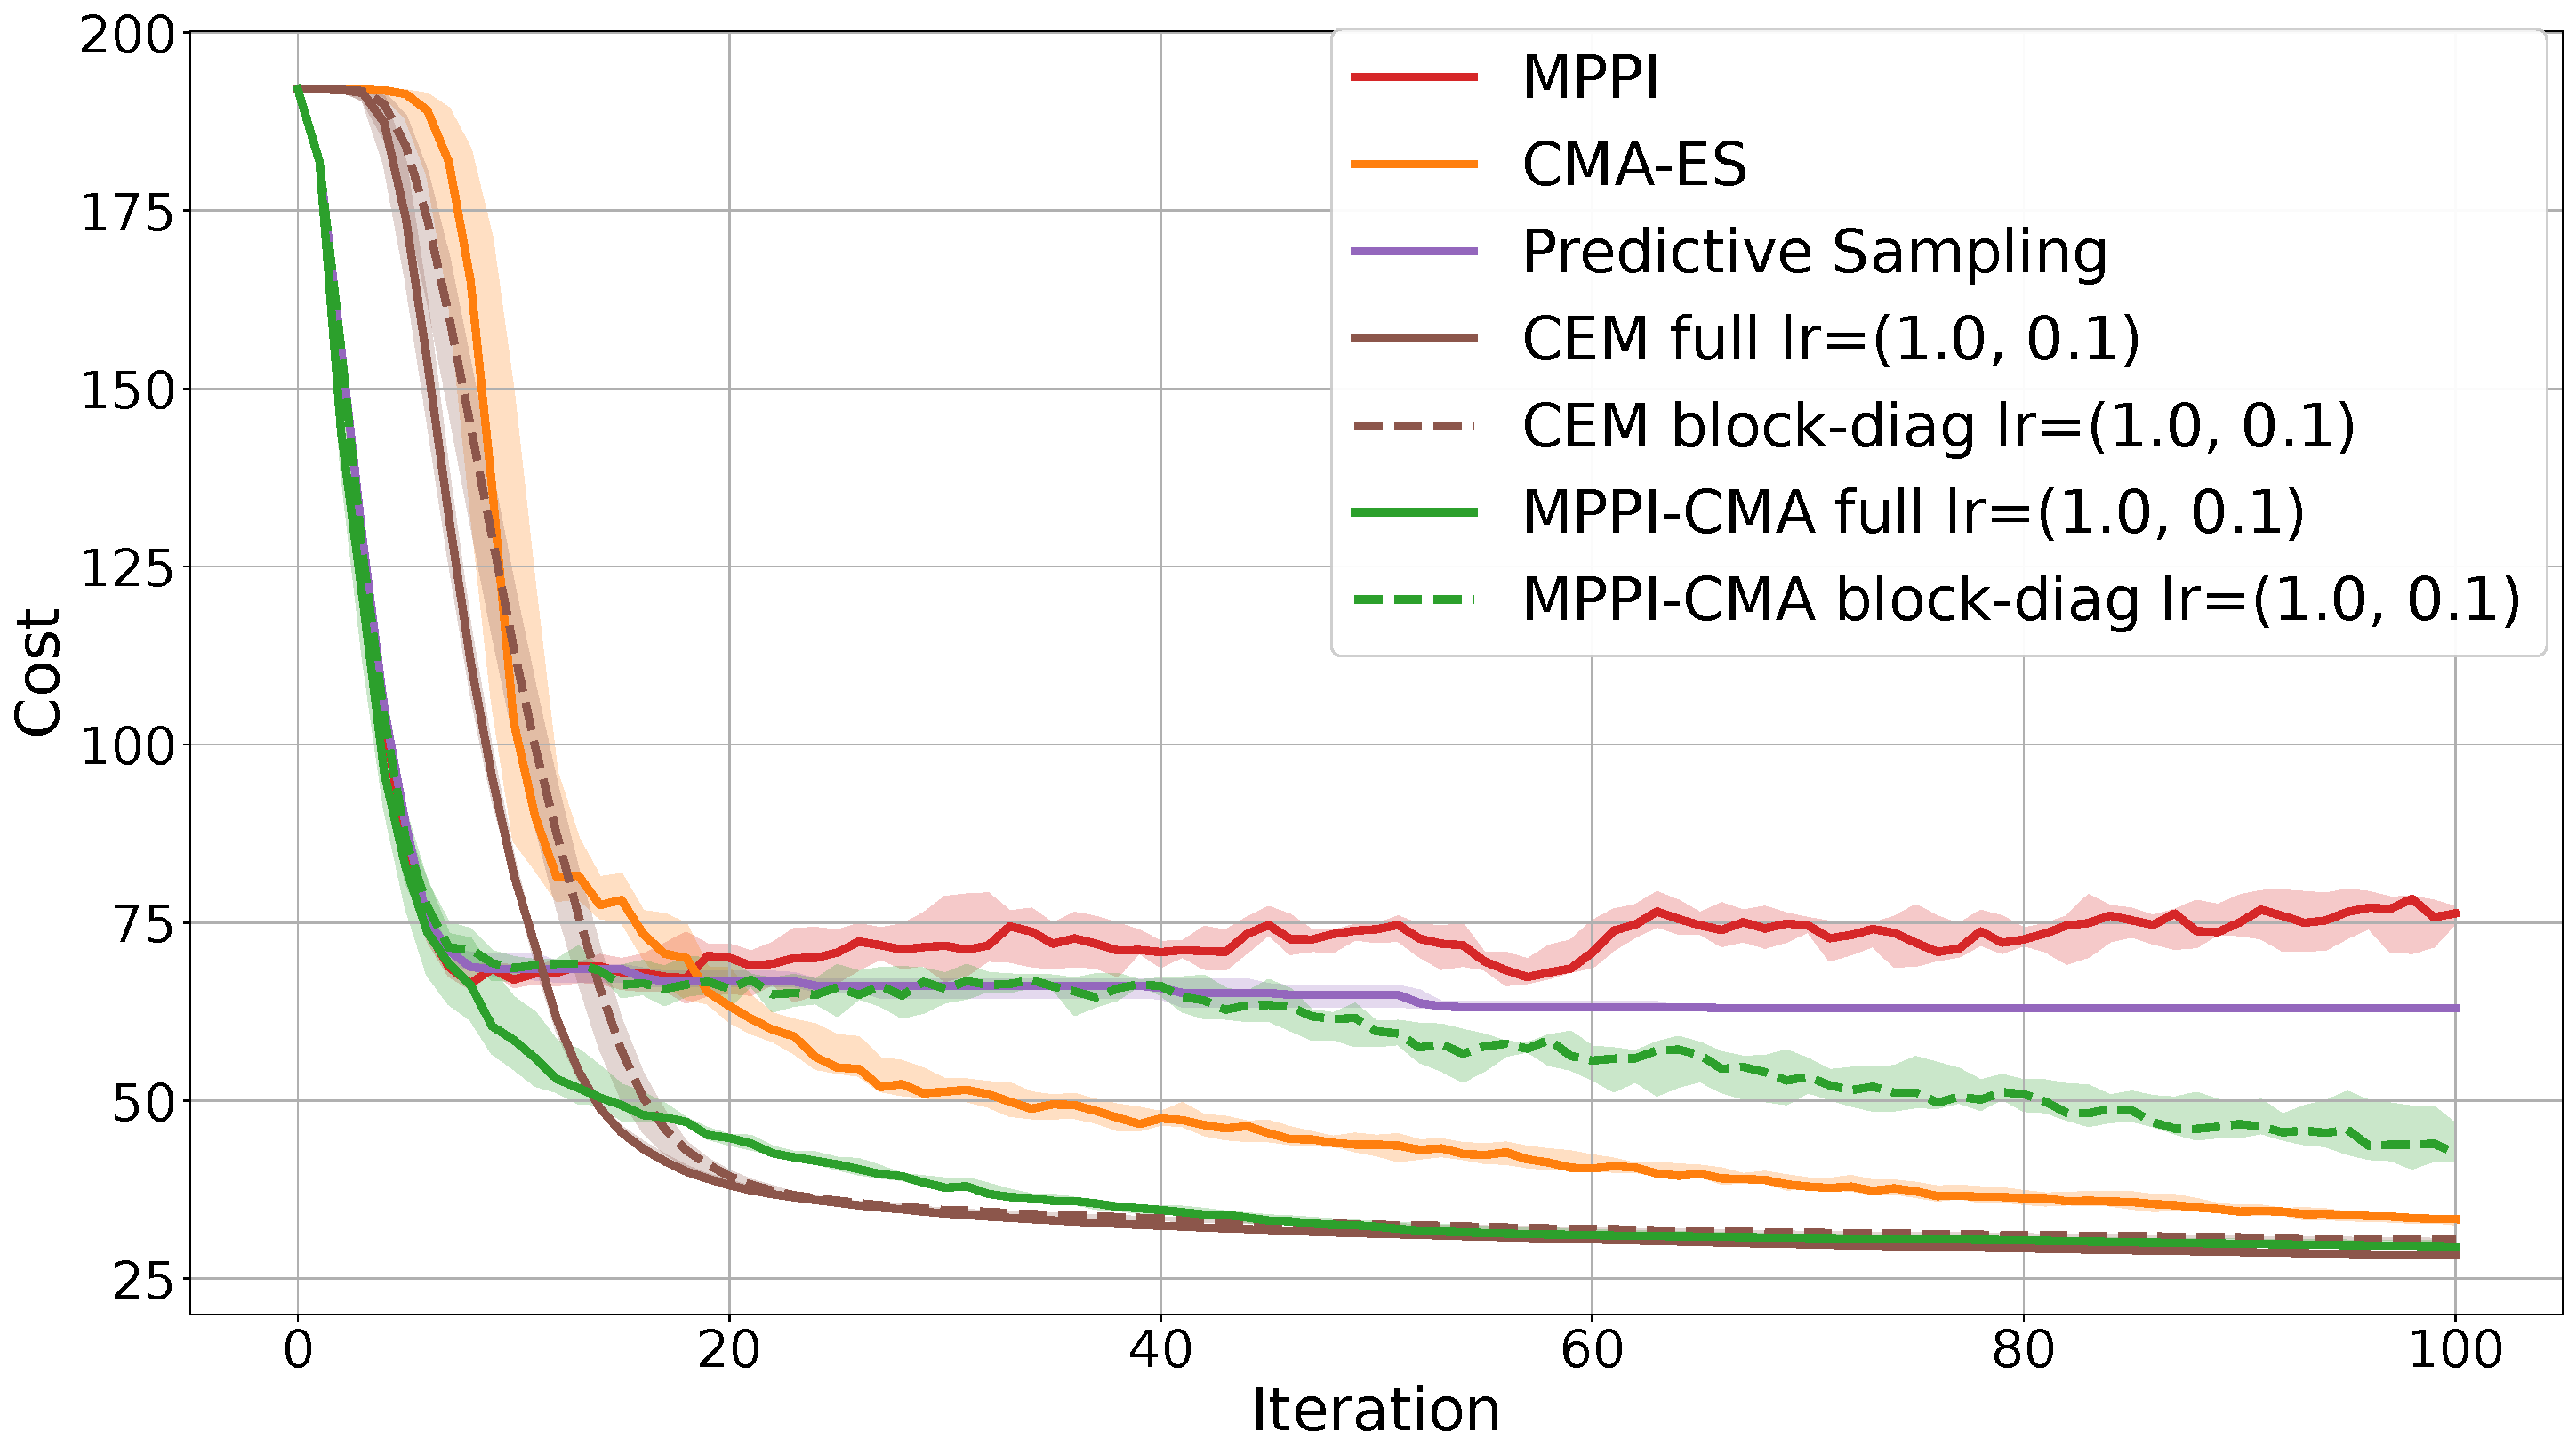
\includegraphics[width=\linewidth]{DoubleCartPoleUnconstrained_Convergence_full.pdf}
  \caption{DoubleCartPole}\end{subfigure}\hfill
\begin{subfigure}{0.32\textwidth}\centering
  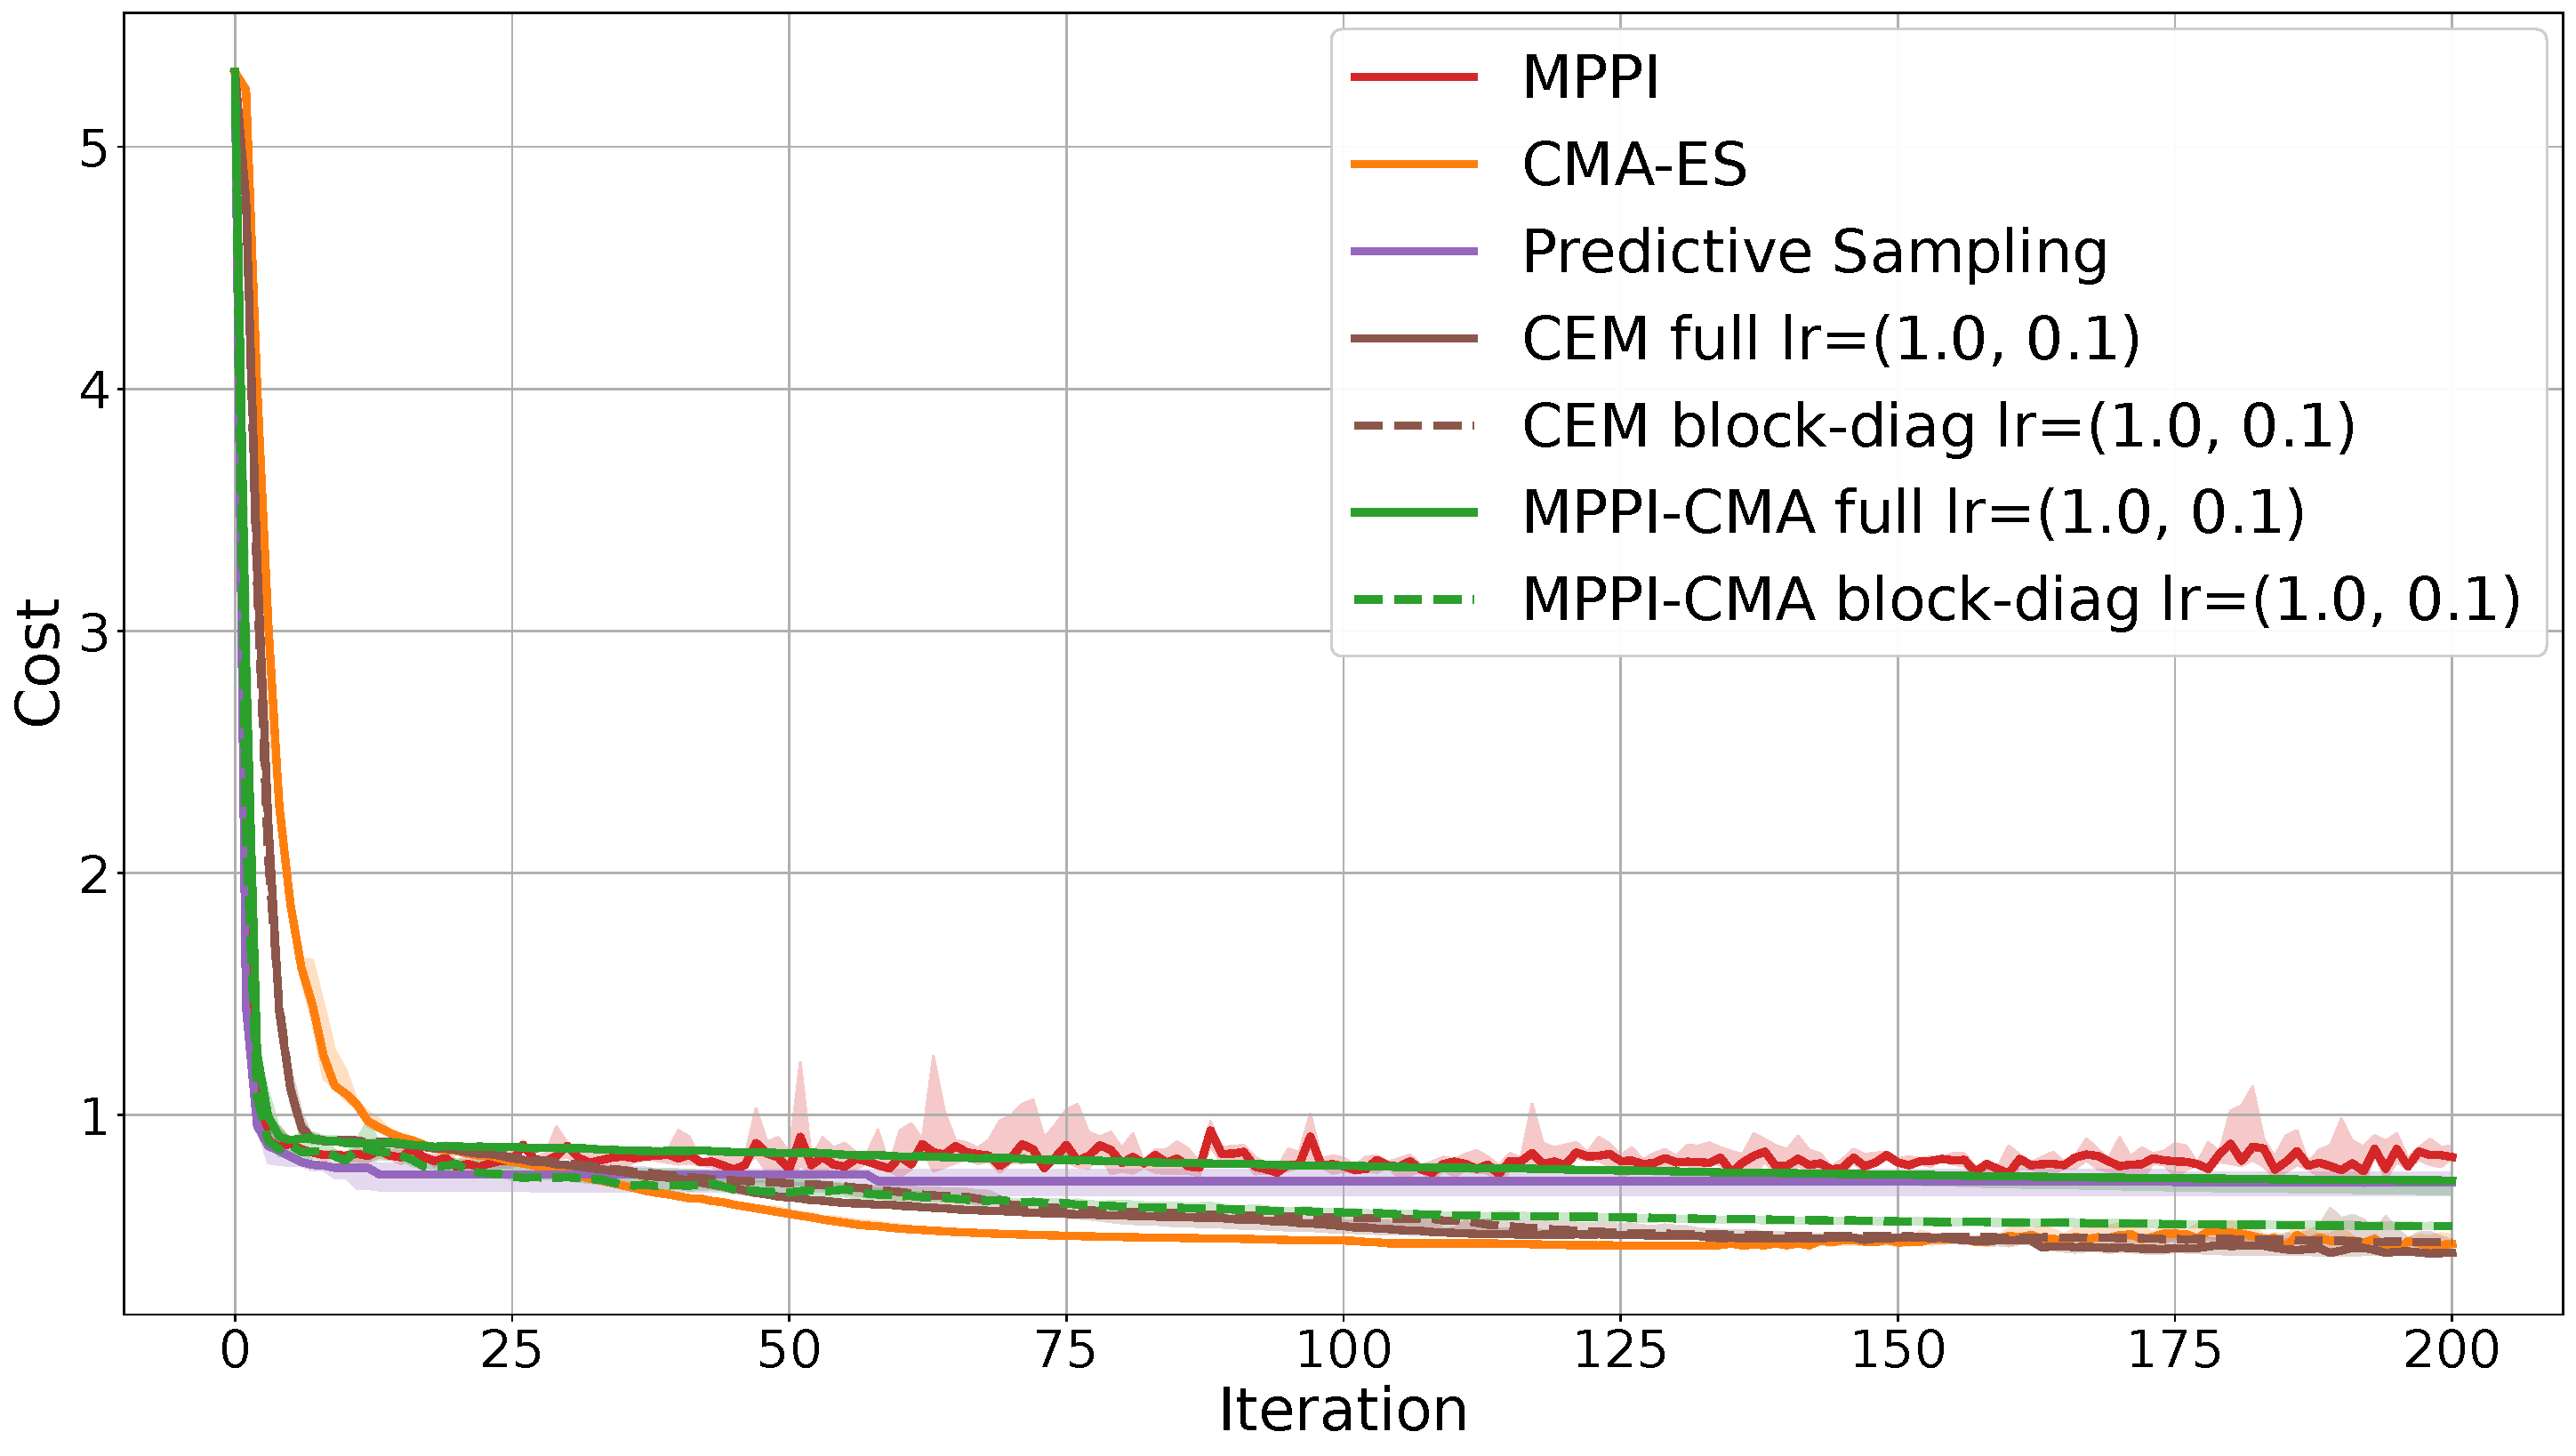
\includegraphics[width=\linewidth]{PushTUnconstrained_Convergence_full.pdf}
  \caption{PushT}\end{subfigure}\\[1.2ex]
% bottom row: humanoid / locomotion
\begin{subfigure}{0.32\textwidth}\centering
  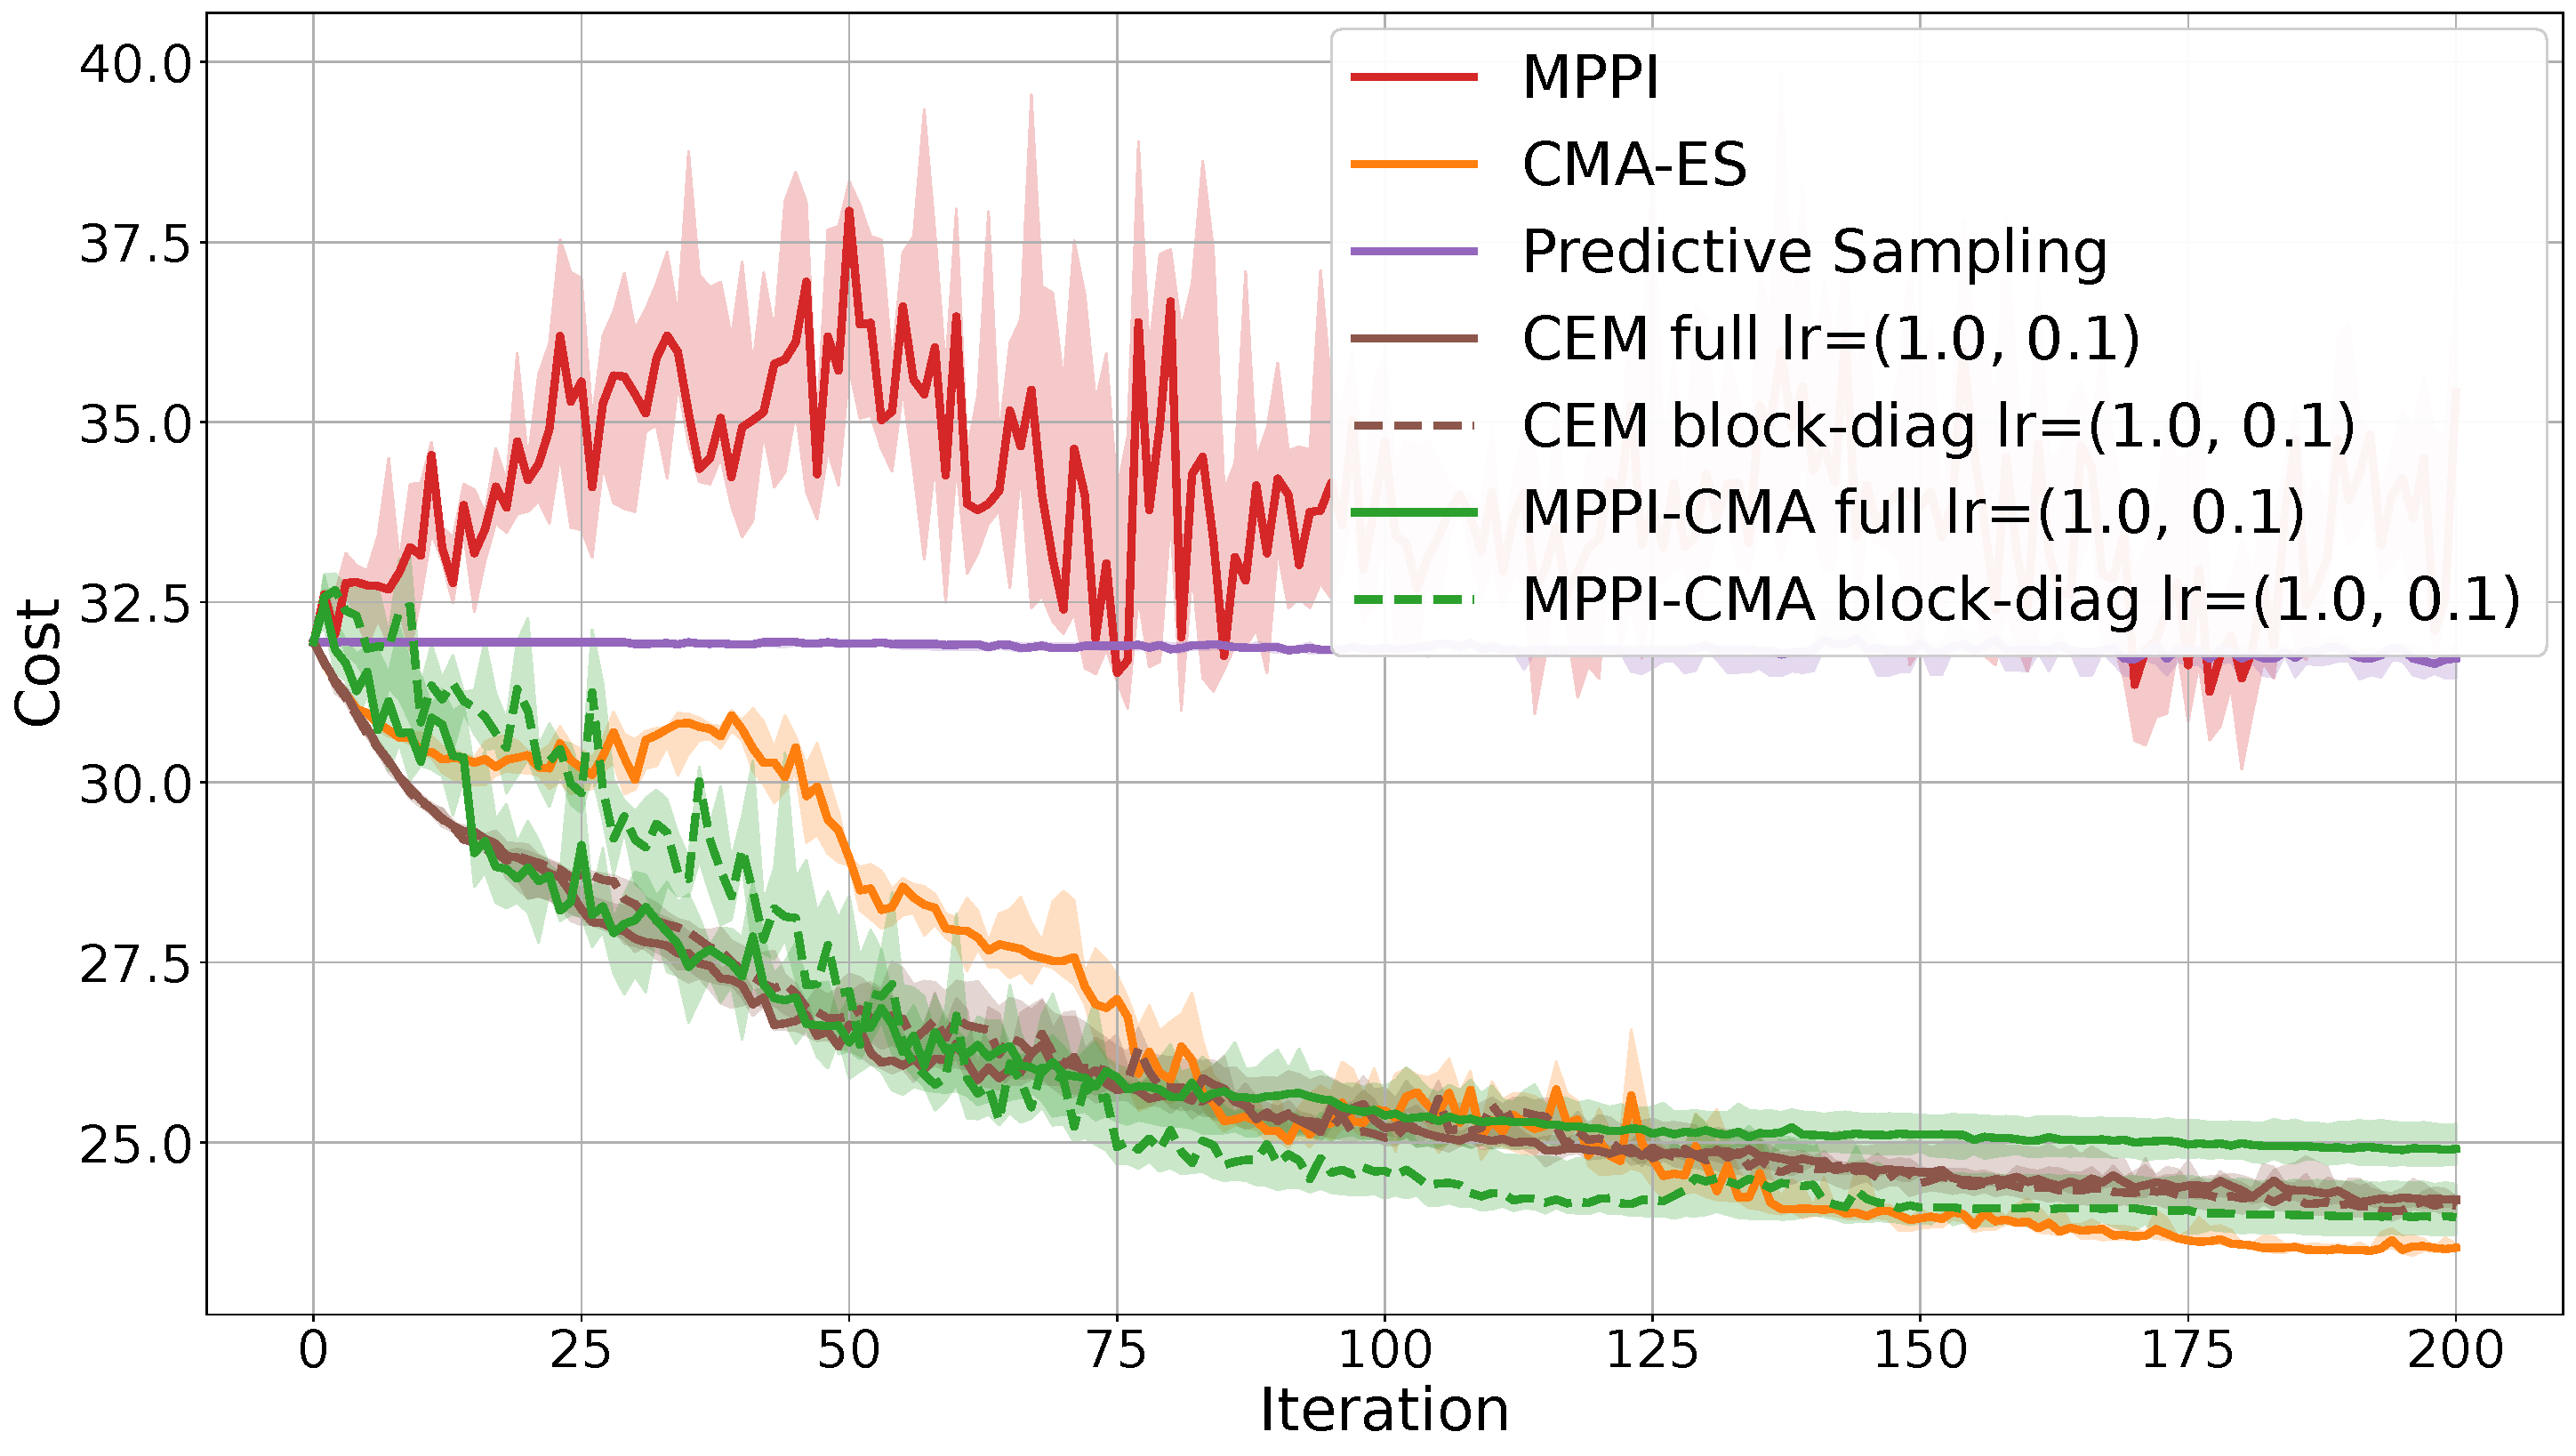
\includegraphics[width=\linewidth]{HumanoidStandupUnconstrained_Convergence_full.pdf}
  \caption{HumanoidStandup}\end{subfigure}\hfill
\begin{subfigure}{0.32\textwidth}\centering
  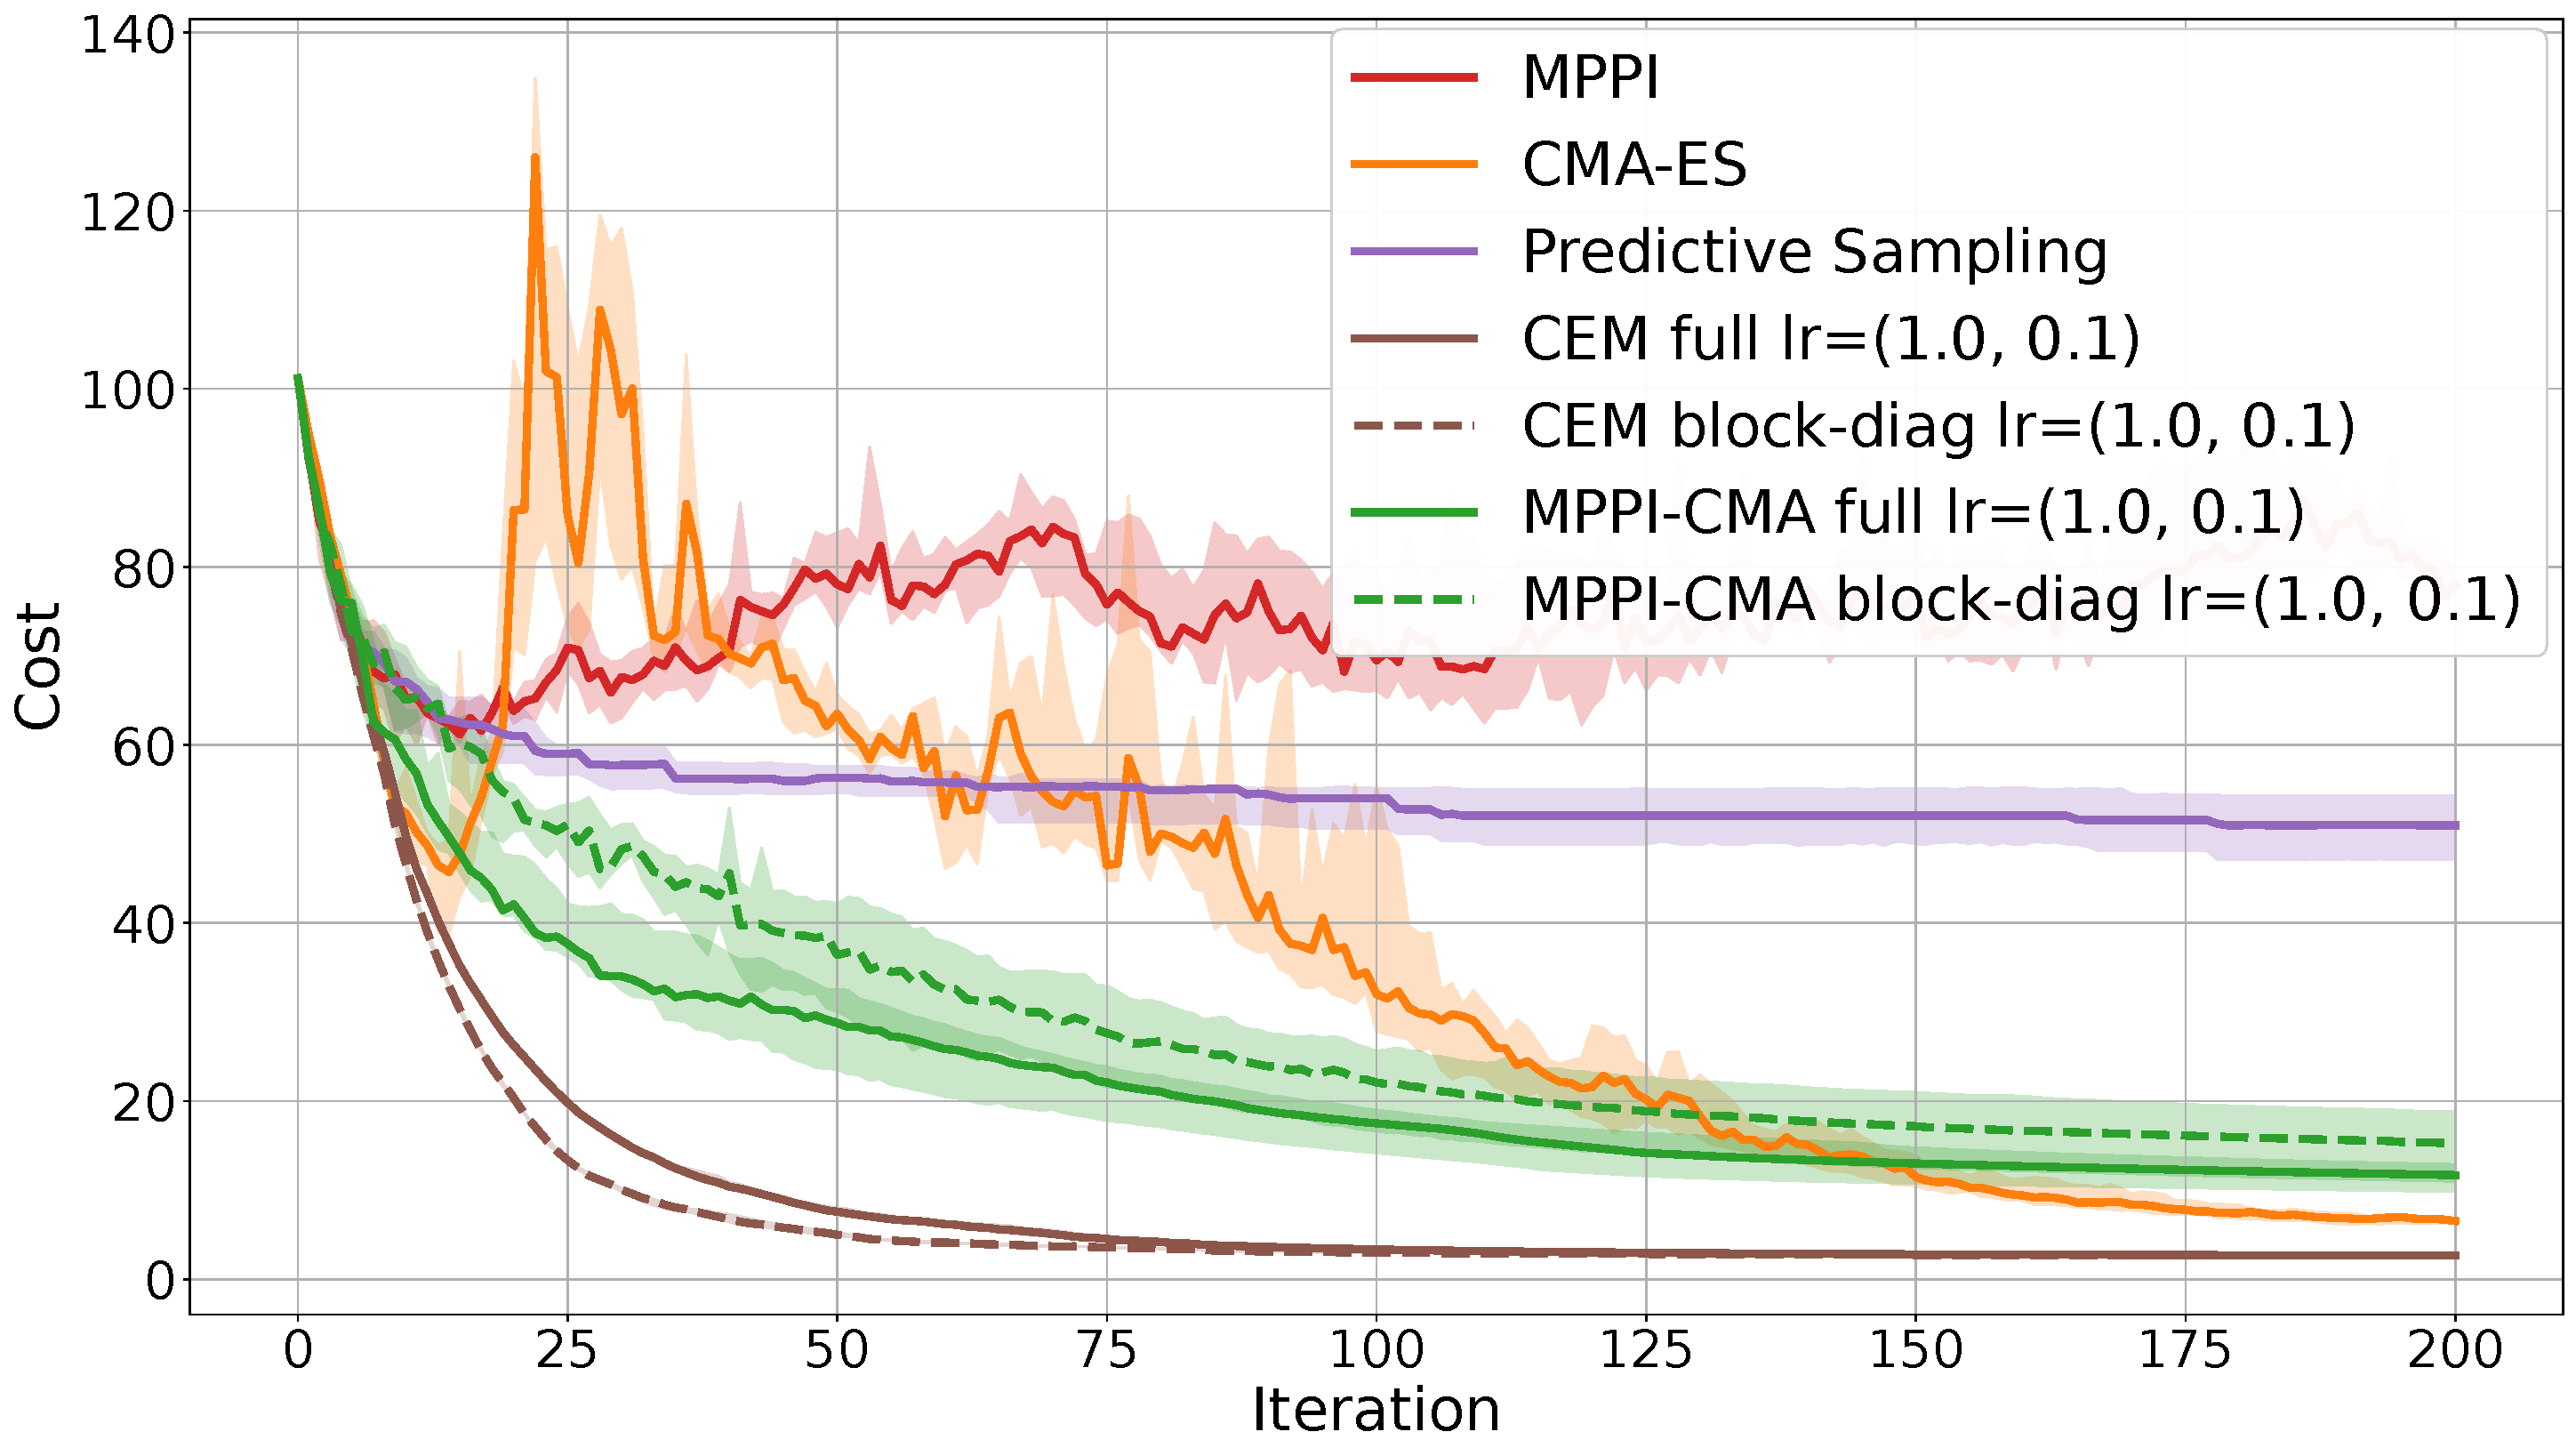
\includegraphics[width=\linewidth]{HumanoidBalanceUnconstrained_Convergence_full.pdf}
  \caption{HumanoidBalance}\end{subfigure}\hfill
\begin{subfigure}{0.32\textwidth}\centering
  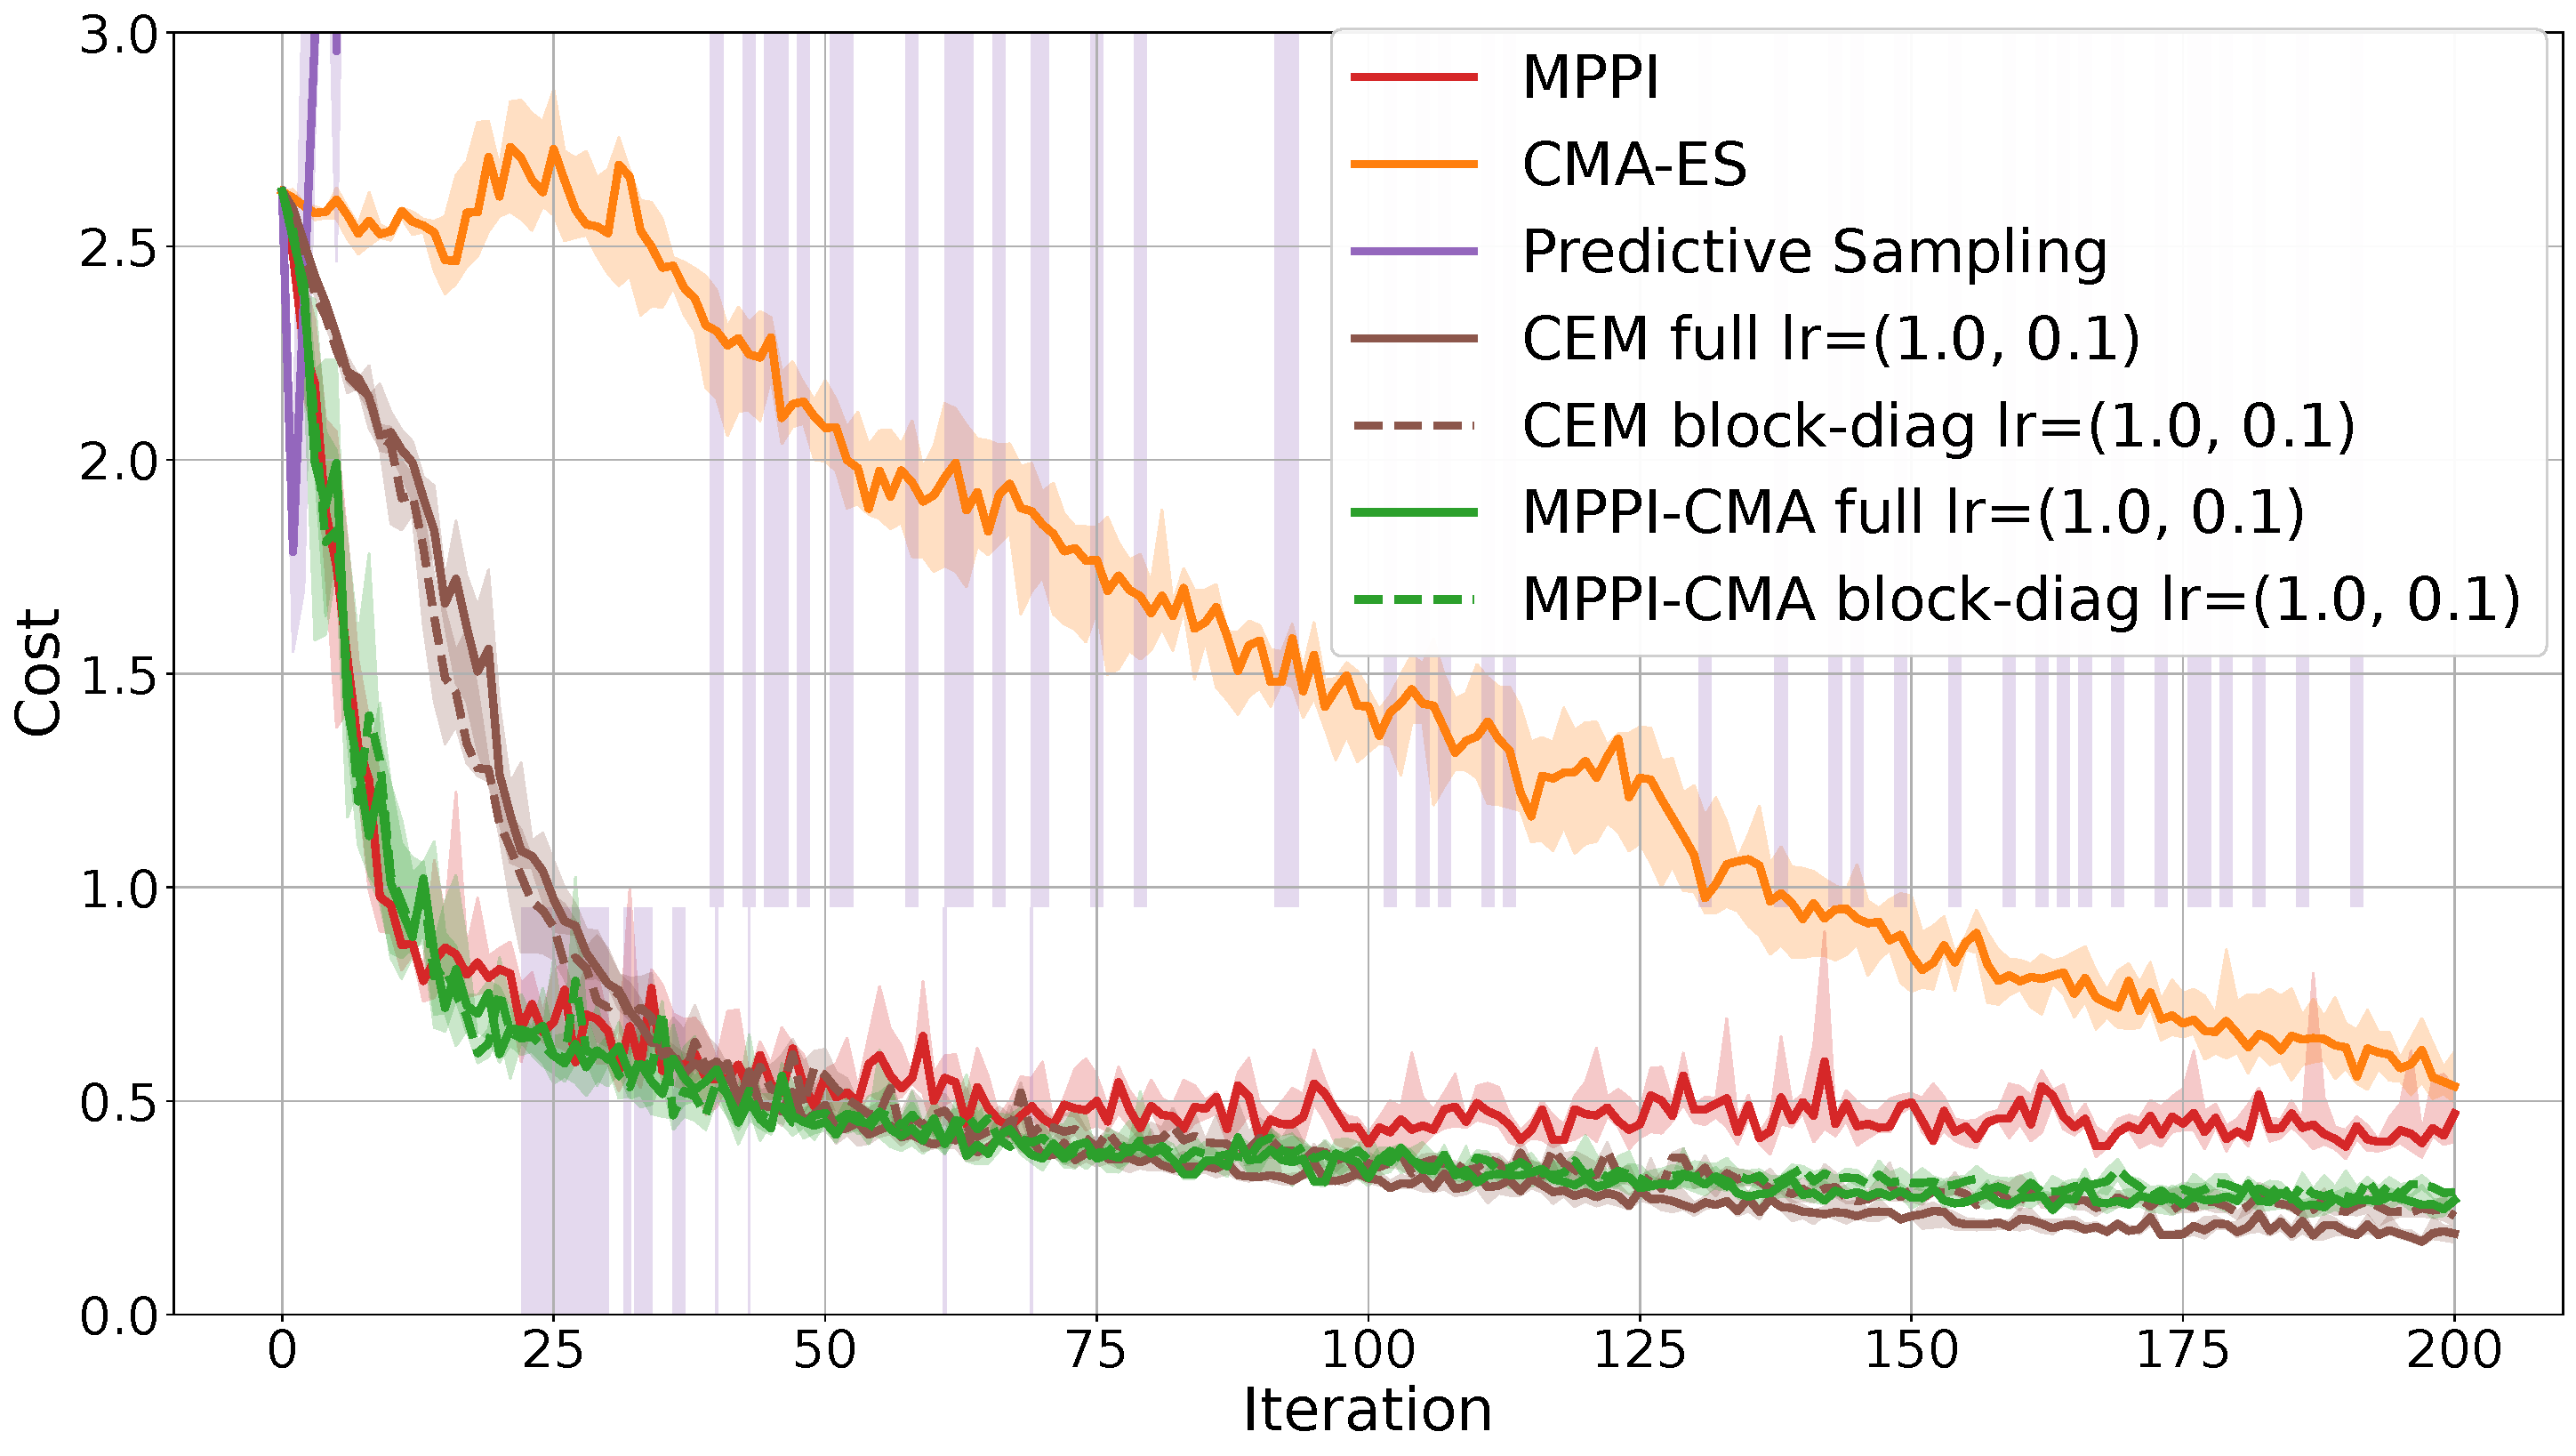
\includegraphics[width=\linewidth]{Go2WalkUnconstrained_Convergence_full.pdf}
  \caption{Go2Walk}\end{subfigure}
\caption{Per-task convergence (appendix, full 7-algorithm set): MPPI, CMA-ES, Predictive Sampling, CEM (full and block-diagonal), and MPPI-CMA (full and block-diagonal), all at $\mathrm{lr}=(1.0, 0.1)$ where applicable; colour denotes the algorithm, dashed = block-diagonal covariance.}
\end{figure}

\end{document}
